\documentclass[11pt,letterpaper]{article}
\usepackage{fontspec}
\setmainfont{texgyrepagella}[Extension=.otf,UprightFont=*-regular,BoldFont=*-bold,ItalicFont=*-italic,BoldItalicFont=*-bolditalic]
\usepackage[bidi=default]{babel}
\babelprovide[import,main]{spanish}
\babelprovide[import]{hebrew}
\babelprovide[import]{ancientgreek}
\babelfont[hebrew]{rm}[Path=fonts/,BoldFont=NotoHebrewSerif-700.ttf,Scale=0.95]{NotoHebrewSerif-400.ttf}
\babelfont[ancientgreek]{rm}[Path=fonts/]{GFSPorson.otf}
\newcommand{\heb}[1]{\mbox{\foreignlanguage{hebrew}{#1}}}
\newcommand{\grc}[1]{\foreignlanguage{ancientgreek}{#1}}
\newcommand{\hebverso}[1]{\par\smallskip{\centering\begin{otherlanguage}{hebrew}\large #1\end{otherlanguage}\par}\smallskip}
\newcommand{\SENOR}{\textsc{Señor}}
\usepackage[margin=2.5cm,headheight=14pt]{geometry}
\usepackage{microtype,ragged2e,booktabs,graphicx,xcolor,csquotes,array}
\usepackage[hidelinks]{hyperref}\usepackage{xurl}\urlstyle{same}
\usepackage[most]{tcolorbox}
\usepackage{tikz}\usetikzlibrary{arrows.meta,positioning,calc,decorations.pathreplacing}
\usepackage{titlesec,fancyhdr}
\definecolor{azul}{HTML}{15437C}\definecolor{azuloscuro}{HTML}{0B1F3A}\definecolor{celeste}{HTML}{5694D6}
\definecolor{dorado}{RGB}{196,154,60}\definecolor{papiro}{RGB}{246,239,220}\definecolor{gris}{RGB}{70,78,96}
\titleformat{\section}{\Large\bfseries\color{azul}}{\thesection.}{0.6em}{}
\titleformat{\subsection}{\large\bfseries\color{azuloscuro}}{\thesubsection}{0.6em}{}
\pagestyle{fancy}\fancyhf{}
\fancyhead[L]{\foreignlanguage{spanish}{\small\itshape\color{gris}La verdad de Dios}}\fancyhead[R]{\foreignlanguage{spanish}{\small\color{gris}\thepage}}
\renewcommand{\headrulewidth}{0.4pt}
\setlength{\parindent}{1.27cm}\linespread{1.15}\setlength{\emergencystretch}{3em}
\newtcolorbox{cita}[1][]{enhanced,colback=azul!6!white,colframe=azul,boxrule=0pt,leftrule=2.5pt,arc=0pt,
  left=8pt,right=8pt,top=5pt,bottom=5pt,before skip=8pt,after skip=8pt,fontupper=\itshape,#1}
\newcommand{\fuente}[1]{\par\hfill{\upshape\bfseries\small\textcolor{azul}{#1}}}
\newtcolorbox{nota}[1][]{enhanced,colback=dorado!10,colframe=dorado!85!azul,boxrule=0.6pt,arc=2pt,
  fonttitle=\bfseries\small,coltitle=azuloscuro,colbacktitle=dorado!30,fontupper=\small,title={#1}}
\newtcolorbox{filologia}[1][]{enhanced,colback=white,colframe=azul!45,boxrule=0.5pt,arc=2pt,
  fonttitle=\bfseries\small,coltitle=white,colbacktitle=azul!80,fontupper=\small,title={Filología: #1}}
\newcommand{\refapa}[1]{\par{\RaggedRight\hangindent=1.27cm\hangafter=1\noindent #1\par}\vspace{4pt}}
\newcommand{\destacar}[1]{\textbf{\textcolor{azul}{#1}}}
\newcolumntype{L}[1]{>{\RaggedRight\arraybackslash}p{#1}}


\title{\color{azul}\bfseries La verdad de Dios\\[4pt]\large\color{gris}\mdseries ``Mas \SENOR{} es el Dios verdadero'' (Jer 10:10)}
\author{}\date{}
\begin{document}
\maketitle\thispagestyle{empty}

\begin{abstract}\noindent
``Toda verdad es verdad de Dios'': este capítulo parte de esa premisa y la ancla en Jeremías 10, donde el profeta opone los ídolos clavados para no caerse al \SENOR{}, que es \emph{Elohim emet}, ``Dios verdad'', vivo y Rey eterno (Jer 10:10). Recorre la raíz hebrea \emph{amán} en sus usos concretos (sostener, cargar, ser firme) y el espectro completo de términos hebreos, arameos y griegos que la Reina-Valera 1960 traduce con ``verdad'', con la imagen bíblica de la plomada (Am 7; Is 28). Define la verdad de Dios como la perfección eterna por la cual Dios es real y firme, dice lo que es y cumple lo que dice, de modo que su palabra corresponde a la realidad que él creó y sostiene. Desde allí examina las esferas de la creación (la ciencia, el gobierno, la economía y la moral) y el choque entre la verdad y la percepción humana, con casos recientes documentados. Presenta un encuentro en la historia de Israel (la viuda de Sarepta), la mirada judía (``el sello del Santo es \emph{emet}'', el Talmud, el midrash, la liturgia, Maimónides y Qumrán) y la lectura de Pablo: la verdad cambiada por la mentira (Ro 1:25), ``sea Dios veraz'' (Ro 3:4), Cristo siervo de la verdad de Dios (Ro 15:8) y el ``Sí'' y el ``Amén'' de todas las promesas (2~Co 1:20). Termina con la verdad como atributo comunicable en su forma de veracidad.
\par\smallskip\noindent\textbf{Palabras clave:} verdad, \emph{emet}, \emph{amán}, Jeremías 10, plomada, \emph{alétheia}, amén, Pablo.\end{abstract}

\begin{nota}[Nota sobre el texto]
Las citas bíblicas son de la Reina-Valera 1960. Donde esta escribe ``Jehová'', aquí se escribe \SENOR, que traduce el tetragrama \heb{יהוה}, leído en la tradición judía como \emph{Adonay}. El hebreo sigue la BHS; el griego, NA28 y la Septuaginta de Rahlfs-Hanhart. Las fuentes judías (Talmud, midrash, Misná, Maimónides) se citan desde Sefaria, y los textos de Qumrán desde las ediciones de García Martínez (1992) y Vermes (2004); todo lo que es interpretación se marca como precisión. Cuando la numeración hebrea difiere de la española se da entre corchetes.
\end{nota}

%===================================================================
\section{Premisa: toda verdad es verdad de Dios}

Desde una cosmovisión bíblica, la verdad no es un constructo social ni una abstracción filosófica. Es la correspondencia exacta entre lo que creemos y la realidad tal como Dios la concibió, la creó y la sostiene. Si Dios es la fuente inagotable de la verdad, cualquier cosa que sea verdadera en el universo proviene de él: la que estudia la física, la que organiza la política y la economía, la que sostiene la moral y la que define al ser humano.

\begin{nota}[Precisión]
La fórmula ``toda verdad es verdad de Dios'' resume una idea que la tradición cristiana remonta a Agustín: el cristiano debe reconocer que dondequiera encuentre la verdad, esta pertenece a su Señor (\emph{De doctrina christiana} II.18.28).
\end{nota}

En el juicio de Jesús, Pilato hace la pregunta que recorre este capítulo:

\begin{cita}Le dijo entonces Pilato: ¿Luego, eres tú rey? Respondió Jesús: Tú dices que yo soy rey. Yo para esto he nacido, y para esto he venido al mundo, para dar testimonio a la verdad. Todo aquel que es de la verdad, oye mi voz. Le dijo Pilato: ¿Qué es la verdad?\fuente{(Jn 18:37--38)}\end{cita}

Pilato pregunta \emph{qué} es la verdad (\grc{τί ἐστιν ἀλήθεια;}) delante de \emph{quién} es la verdad (Jn 14:6). El estudio sigue ese mismo camino en cuatro pasos: qué es la verdad y de dónde viene su firmeza; en qué esferas de la creación se descubre; cómo choca con la percepción humana; y cómo se revela, al fin, como una Persona.

La conexión con el verso que une esta obra es directa. Jeremías escribe: ``Mas alábese en esto el que se hubiere de alabar: en entenderme y conocerme, que yo soy \SENOR'' (Jer 9:24 [9:23]). Pocos versos después, el mismo libro dice quién es ese Dios que puede ser conocido: ``Mas \SENOR{} es el Dios verdadero'' (Jer 10:10).

%===================================================================
\section{Texto ancla: Jeremías 10:10}\label{sec:jer10}

\subsection{Ídolos que no hablan}
Jeremías 10:1--16 es una sátira contra los ídolos de las naciones. Jeremías describe el proceso de fabricación con ironía:

\begin{cita}Porque las costumbres de los pueblos son vanidad; porque leño del bosque cortaron, obra de manos de artífice con buril. Con plata y oro lo adornan; con clavos y martillo lo afirman para que no se mueva. Derechos están como palmera, y no hablan; son llevados, porque no pueden andar. No tengáis temor de ellos, porque ni pueden hacer mal, ni para hacer bien tienen poder.\fuente{(Jer 10:3--5)}\end{cita}

El ídolo necesita clavos para quedarse firme. Su estabilidad es prestada: alguien lo sostiene, alguien lo carga, alguien lo viste (10:9). No habla, no anda y no puede hacer ni mal ni bien. Jeremías lo llama ``vanidad'' (\heb{הֶבֶל}, \emph{hével}), la palabra del vapor y del soplo que tanto usa Eclesiastés.

\begin{nota}[Precisión]
El contraste entre la ``firmeza clavada'' del ídolo y la firmeza de Dios (\emph{emet}) es una lectura propia de esta serie, sugerida por el verbo \heb{יְחַזְּקוּם} (``lo afirman'', 10:4) y por la raíz de \emph{emet}.
\end{nota}

\subsection{El Dios verdadero}
En medio de esa descripción, el poema confiesa:

\hebverso{וַיהוָה אֱלֹהִים אֱמֶת הוּא־אֱלֹהִים חַיִּים וּמֶלֶךְ עוֹלָם \\ מִקִּצְפּוֹ תִּרְעַשׁ הָאָרֶץ וְלֹא־יָכִלוּ גוֹיִם זַעְמוֹ}
\begin{cita}Mas \SENOR{} es el Dios verdadero; él es Dios vivo y Rey eterno; a su ira tiembla la tierra, y las naciones no pueden sufrir su indignación.\fuente{(Jer 10:10)}\end{cita}

\begin{filologia}[Jer 10:10]
\begin{tabular}{@{}L{3.2cm}L{1.6cm}L{10cm}@{}}
\heb{אֱלֹהִים אֱמֶת} \emph{Elohim emet} & \heb{אמן} & ``Dios verdad'': el sustantivo \emph{emet} se pone junto a \emph{Elohim} para calificarlo. No dice que Dios \emph{tenga} verdad, sino que \emph{es} verdad. \\[2pt]
\heb{אֱלֹהִים חַיִּים} \emph{Elohim jayyim} & \heb{חיה} & ``Dios vivo'': frente al ídolo, en el que ``no hay espíritu'' (10:14). \\[2pt]
\heb{מֶלֶךְ עוֹלָם} \emph{mélej olam} & \heb{מלך} & ``Rey eterno'': al ídolo lo llevan (10:5); el \SENOR{} gobierna. \\[2pt]
\heb{כִּי שֶׁקֶר נִסְכּוֹ} \emph{ki shéqer nisko} & \heb{שׁקר} & ``porque mentira es su imagen fundida'' (10:14). El ídolo es \emph{shéqer}, lo contrario de \emph{emet}. \\
\end{tabular}
\end{filologia}

El capítulo opone dos realidades: el Dios que \emph{es} verdad y la imagen que \emph{es} mentira. ``Todo hombre se embrutece, y le falta ciencia; se avergüenza de su ídolo todo fundidor, porque mentirosa es su obra de fundición, y no hay espíritu en ella'' (Jer 10:14). La mentira, en Jeremías, no es primero una frase falsa: es un dios falso. Pablo usará el mismo lenguaje (Ro 1:25).

\subsection{Dos columnas que se alternan}
El poema avanza como un juicio con dos voces. Cada descripción de los ídolos recibe una respuesta sobre el Dios verdadero:

\begin{center}\small\renewcommand{\arraystretch}{1.2}
\begin{tabular}{@{}L{3.0cm}L{4.4cm}L{3.0cm}L{4.0cm}@{}}
\toprule
\textbf{Los ídolos} & & \textbf{El \SENOR} & \\ \midrule
vv. 2--5 & leño, clavos, no habla & vv. 6--7 & ``no hay semejante a ti'' \\
vv. 8--9 & ``enseñanza de vanidades'' & v. 10 & Dios verdad, vivo, Rey eterno \\
v. 11 & los dioses desaparecerán & vv. 12--13 & hizo la tierra con su poder \\
vv. 14--15 & mentira, sin espíritu & v. 16 & ``la porción de Jacob'' \\
\bottomrule
\end{tabular}\par
{\footnotesize\color{gris}\textit{Tabla 1.} La alternancia de Jeremías 10:1--16. \textit{Nota.} Elaboración propia.}
\end{center}

El versículo 11 está escrito en arameo, la lengua internacional del imperio:

\hebverso{אֱלָהַיָּא דִּי־שְׁמַיָּא וְאַרְקָא לָא עֲבַדוּ}

\noindent ``los dioses que no hicieron los cielos ni la tierra''. Es la frase que Israel debía decir a las naciones en su propio idioma.

\begin{nota}[Precisión]
La estructura alternada del poema y el carácter arameo del v. 11 se describen en los comentarios (Lundbom, 1999).
\end{nota}

\begin{nota}[Precisión textual]
La Septuaginta de Jeremías es alrededor de una séptima parte más breve que el texto masorético. En el capítulo 10 no tiene los vv. 6--8 ni el v. 10, y pone el v. 9 después del 5a. En Qumrán se encontraron las dos formas: 4QJer\textsuperscript{b} (4Q71) coincide con la forma corta y el orden de la LXX, y 4QJer\textsuperscript{a} (4Q70) sigue la forma larga del texto masorético (Tov, 2012). La RVR1960 sigue el texto masorético, que incluye la confesión del v. 10. Su contenido, en todo caso, está en el resto de la Escritura: ``Dios vivo'' (Dt 5:26; Sal 42:2) y ``Dios de verdad'' (Sal 31:5; Is 65:16).
\end{nota}

%===================================================================
\section{La palabra: la raíz de la firmeza}

\subsection{La raíz \emph{amán} en lo concreto}
En el hebreo bíblico, la palabra para ``verdad'' es \emph{emet} (\heb{אֱמֶת}), de la raíz \heb{א־מ־ן} (\emph{amán}). Esta raíz comunica una realidad física y estructural: sostener, ser firme, construir sobre cimientos sólidos. De ella viene ``amén''. Los usos concretos lo muestran:

\begin{center}\small\renewcommand{\arraystretch}{1.18}
\begin{tabular}{@{}L{3.3cm}L{7.4cm}L{3.6cm}@{}}
\toprule
\textbf{Forma} & \textbf{Uso concreto} & \textbf{Texto} \\ \midrule
\heb{הָאֹמֵן} \emph{ha'omén} & ``la que cría'': el que carga al niño en su seno & Nm 11:12 \\
\heb{אֹמֶנֶת} \emph{oménet} & ``aya'', nodriza: Noemí con el hijo de Rut & Rt 4:16 \\
\heb{אֹמְנוֹת} \emph{omnot} & ``quiciales'', los soportes de las puertas del templo & 2~R 18:16 \\
\heb{אֱמוּנָה} \emph{emuná} & ``firmeza'' de las manos de Moisés sostenidas por Aarón y Hur & Éx 17:12 \\
\heb{נֶאֱמָן} \emph{ne'emán} & ``lugar firme'' donde se clava una estaca & Is 22:23 \\
\heb{וְנֶאְמַן} \emph{vene'mán} & ``será afirmada'' la casa de David & 2~S 7:16 \\
\bottomrule
\end{tabular}\par
{\footnotesize\color{gris}\textit{Tabla 2.} Usos concretos de la raíz \emph{amán}. \textit{Nota.} Textos de la RVR1960 y la BHS.}
\end{center}

\begin{cita}Y las manos de Moisés se cansaban; por lo que tomaron una piedra, y la pusieron debajo de él, y se sentó sobre ella; y Aarón y Hur sostenían sus manos, el uno de un lado y el otro de otro; así hubo en sus manos firmeza hasta que se puso el sol.\fuente{(Éx 17:12)}\end{cita}

La raíz dice sostener y ser sostenido: el brazo que carga a un niño, el poste que sostiene una puerta, las manos que no caen. Lo verdadero es lo que aguanta el peso que se le pone encima.

\begin{nota}[Precisión]
El sentido de una palabra lo fija su uso en contexto, no su etimología; deducir el significado desde la raíz es la ``falacia de la raíz'' (Carson, 2013). En este caso los usos concretos confirman la idea de firmeza que el material de la serie asigna a \emph{emet}; aun así, en cada texto el contexto decide si \emph{emet} significa ``verdad'', ``fidelidad'' o ``seguridad''.
\end{nota}

\subsection{Creer es apoyarse en lo firme}
Isaías juega con la misma raíz en una frase célebre:

\hebverso{אִם לֹא תַאֲמִינוּ כִּי לֹא תֵאָמֵנוּ}
\begin{cita}Si vosotros no creyereis, de cierto no permaneceréis.\fuente{(Is 7:9)}\end{cita}

\begin{filologia}[Is 7:9]
\begin{tabular}{@{}L{3.2cm}L{1.6cm}L{10cm}@{}}
\heb{תַאֲמִינוּ} \emph{ta'aminu} & \heb{אמן} & hifil: ``os apoyáis, creéis''. Creer es apoyar el peso en algo firme. \\[2pt]
\heb{תֵאָמֵנוּ} \emph{te'amenu} & \heb{אמן} & nifal: ``seréis sostenidos, quedaréis firmes''. \\
\end{tabular}
\end{filologia}

``Si no os afirmáis, no seréis afirmados.'' Verdad, fe y fidelidad son ramas de un mismo tronco: \emph{emet} es lo que sostiene, \emph{he'emín} es apoyarse en ello y \emph{emuná} es la firmeza de quien sostiene y de quien se apoya. Por eso, en la Biblia, la fe no se opone a la verdad: la fe se apoya en lo verdadero.

\begin{nota}[Precisión textual]
La Septuaginta lee aquí otra cosa: \grc{καὶ ἐὰν μὴ πιστεύσητε, οὐδὲ μὴ συνῆτε}, ``y si no creéis, tampoco entenderéis''. El juego de palabras solo existe en hebreo.
\end{nota}

\subsection{El espectro completo}
Una sola palabra española, ``verdad'', traduce en la RVR1960 varios términos del original; y una sola raíz hebrea se traduce con varias palabras españolas. En la RVR1960, ``verdad'' y sus formas (``verdadero'', ``verdaderamente'', ``veraz'') aparecen 432 veces en 406 versículos: 188 en el Antiguo Testamento y 244 en el Nuevo.

\begin{center}\small\renewcommand{\arraystretch}{1.16}
\begin{tabular}{@{}L{3.6cm}L{1.1cm}L{5.4cm}L{4.2cm}@{}}
\toprule
\textbf{Término} & \textbf{Veces} & \textbf{Traducción en la RVR1960} & \textbf{Textos} \\ \midrule
\heb{אֱמֶת} \emph{emet} & 127 & ``verdad'' ($\approx$\,93), ``verdadero/a'' (9), ``fidelidad'' (4), ``seguridad'', ``rectamente'' & Gn 24:27; Jer 10:10; Sal 31:5 \\
\heb{אֱמוּנָה} \emph{emuná} & 49 & ``verdad'' (18), ``fidelidad'' (13), ``firmeza'', ``fe'' & Éx 17:12; Dt 32:4; Hab 2:4 \\
\heb{אָמֵן} \emph{amén} & 30 & ``amén'' (28); ``Dios de verdad'' (2) & Dt 27:15; Is 65:16 \\
\heb{אֹמֶן} \emph{ómen} & 1 & ``firmeza'' & Is 25:1 \\
\heb{אָמְנָם}, \heb{אֻמְנָם} \emph{omnam} & 14 & ``verdaderamente'', ``de veras'' & 1~R 8:27; Job 19:4 \\
\heb{אָכֵן} \emph{ajén} & --- & ``verdaderamente'' & Is 45:15 \\
\heb{נָכוֹן} \emph{najón} & --- & ``cosa cierta'' (junto a \emph{emet}) & Dt 13:14; 17:4 \\
\heb{קֹשֶׁט} \emph{qóshet} & 2 & ``verdad'' & Pr 22:21 \\
arameo \heb{קְשֹׁט} \emph{qeshot} & 2 & ``verdaderas'', ``ciertamente'' & Dn 2:47; 4:37 \\
arameo \heb{יַצִּיב} \emph{yatsiv} & 5 & ``verdadero'', ``la verdad'' & Dn 2:45; 7:16 \\ \midrule
\grc{ἀλήθεια} \emph{alétheia} & 109 & ``verdad'' (104) & Jn 14:6; Ro 1:25 \\
\grc{ἀληθής} \emph{alēthés} & 26 & ``verdadero'', ``veraz'' & Jn 8:26; Ro 3:4 \\
\grc{ἀληθινός} \emph{alēthinós} & 28 & ``verdadero'' (genuino, real) & Jn 15:1; 1~Ts 1:9 \\
\grc{ἀληθῶς} \emph{alēthós} & 18 & ``verdaderamente'' & 1~Ts 2:13 \\
\grc{ἀληθεύω} \emph{alētheúō} & 2 & ``decir la verdad'', ``seguir la verdad'' & Gá 4:16; Ef 4:15 \\
\grc{ἀψευδής} \emph{apseudés} & 1 & ``que no miente'' & Tit 1:2 \\
\grc{ἀμήν} \emph{amén} & 128 & ``de cierto'', ``amén'' & 2~Co 1:20; Ap 3:14 \\ \midrule
\heb{שֶׁקֶר} \emph{shéqer} & 113 & ``mentira, falsedad, engaño'' & Jer 10:14; 28:15 \\
\heb{כָּזָב} \emph{kazav} & 31 & ``mentira''; el verbo: ``mentir'' & Sal 116:11; Is 28:17 \\
\grc{ψεῦδος}, \grc{ψεύστης} & 10; 10 & ``mentira''; ``mentiroso'' & Ro 1:25; Jn 8:44 \\
\bottomrule
\end{tabular}\par
{\footnotesize\color{gris}\textit{Tabla 3.} El espectro de ``verdad''. \textit{Nota.} Conteo propio con la BHS y NA27 con números Strong, y la RVR1960 sin títulos de sección.}
\end{center}

\begin{nota}[Precisión]
Los conteos son propios y conviene verificarlos en una concordancia (e-Sword). No se da cifra para \emph{ajén} y \emph{najón} porque en la mayoría de sus usos no significan ``verdad''. Además, la RVR1960 usa 57 veces el giro ``a la verdad'', que casi siempre traduce la partícula griega \grc{μέν} (``por cierto'') y no habla de la verdad como tema.
\end{nota}

\subsection{Una palabra, dos traducciones}
Como \emph{emet} y \emph{emuná} unen verdad y fidelidad, las versiones eligen a veces un lado y a veces el otro. El compendio del material de la serie lo muestra:

\begin{center}\small\renewcommand{\arraystretch}{1.2}
\begin{tabular}{@{}L{1.8cm}L{2.4cm}L{3.3cm}L{3.2cm}L{3.4cm}@{}}
\toprule
\textbf{Texto} & \textbf{Original} & \textbf{RVR1960} & \textbf{LBLA} & \textbf{NVI} \\ \midrule
Sal 119:30 & \heb{דֶּרֶךְ־אֱמוּנָה} & ``el camino de la verdad'' & ``el camino de la verdad'' & ``el camino de la fidelidad'' \\
Sal 119:160 & \heb{רֹאשׁ־דְּבָרְךָ אֱמֶת} & ``La suma de tu palabra es verdad'' & ``La suma de tu palabra es verdad'' & ``La suma de tus palabras es la verdad'' \\
Jer 5:1 & \heb{מְבַקֵּשׁ אֱמוּנָה} & ``que busque verdad'' & ``que busque la verdad'' & ``y busque la verdad'' \\
3~Jn 3 & \grc{τῇ ἀληθείᾳ} & ``tu verdad'' & ``tu verdad'' & ``tu fidelidad'' \\
\bottomrule
\end{tabular}\par
{\footnotesize\color{gris}\textit{Tabla 4.} Verdad y fidelidad en tres versiones. \textit{Nota.} NVI y LBLA según el compendio de la serie y la biblioteca bíblica.}
\end{center}

Las versiones no se contradicen; eligen uno de los dos lados de la misma raíz. En hebreo, ser verdadero es ser confiable. El caso de Sal 119:160 tiene otro matiz: \heb{רֹאשׁ} (\emph{rosh}) es ``cabeza'', y puede entenderse como ``la suma'' (el total, como al contar cabezas) o como ``el principio''. La RVR1960 traduce ``La suma de tu palabra es verdad''; la RV1909 y el material de la serie, ``El principio de tu palabra es verdad''. Las dos lecturas afirman que la palabra de Dios es verdad de punta a punta.

\subsection{La primera vez: el siervo de Abraham}
La primera aparición de \emph{emet} en la Biblia llega en pareja con \emph{jésed}. El siervo de Abraham ora pidiendo una señal para encontrar esposa a Isaac (Gn 24:12--14), y Dios responde tal como él pidió:

\hebverso{בָּרוּךְ יְהוָה אֱלֹהֵי אֲדֹנִי אַבְרָהָם אֲשֶׁר לֹא־עָזַב חַסְדּוֹ וַאֲמִתּוֹ מֵעִם אֲדֹנִי}
\begin{cita}y dijo: Bendito sea \SENOR{}, Dios de mi amo Abraham, que no apartó de mi amo su misericordia y su verdad, guiándome \SENOR{} en el camino a casa de los hermanos de mi amo.\fuente{(Gn 24:27)}\end{cita}

Más adelante repite que Dios lo guió ``por camino de verdad'' (\heb{בְּדֶרֶךְ אֱמֶת}, Gn 24:48): el camino correcto, el que llega a destino. La verdad, en su primera aparición, es la de un Dios que guía y cumple.

\subsection{El Dios del Amén}
\hebverso{הַמִּתְבָּרֵךְ בָּאָרֶץ יִתְבָּרֵךְ בֵּאלֹהֵי אָמֵן \\ וְהַנִּשְׁבָּע בָּאָרֶץ יִשָּׁבַע בֵּאלֹהֵי אָמֵן}
\begin{cita}El que se bendijere en la tierra, en el Dios de verdad se bendecirá; y el que jurare en la tierra, por el Dios de verdad jurará; porque las angustias primeras serán olvidadas, y serán cubiertas de mis ojos.\fuente{(Is 65:16)}\end{cita}

\begin{filologia}[Is 65:16]
\begin{tabular}{@{}L{3.2cm}L{1.6cm}L{10cm}@{}}
\heb{אֱלֹהֵי אָמֵן} \emph{Elohé amén} & \heb{אמן} & literalmente ``el Dios del Amén''. La RVR1960 traduce ``Dios de verdad''. \\[2pt]
\grc{τὸν θεὸν τὸν ἀληθινόν} & --- & la Septuaginta traduce ``el Dios verdadero'', con el adjetivo que Pablo usará en 1~Ts 1:9. \\
\end{tabular}
\end{filologia}

El texto está en el anuncio de los cielos nuevos y la tierra nueva (Is 65:17). Dios dice ``amén'' a su propia palabra: lo que promete, es. Esta expresión prepara el título que el Apocalipsis da a Cristo: ``He aquí el Amén, el testigo fiel y verdadero'' (Ap 3:14).

\subsection{Lo que permanece y lo que dura un momento}
\hebverso{שְׂפַת־אֱמֶת תִּכּוֹן לָעַד וְעַד־אַרְגִּיעָה לְשׁוֹן שָׁקֶר}
\begin{cita}El labio veraz permanecerá para siempre; Mas la lengua mentirosa sólo por un momento.\fuente{(Pr 12:19)}\end{cita}

\begin{filologia}[Pr 12:19]
\begin{tabular}{@{}L{3.2cm}L{1.6cm}L{10cm}@{}}
\heb{שְׂפַת־אֱמֶת} \emph{sefat emet} & \heb{אמן} & ``labio de verdad''. \\[2pt]
\heb{תִּכּוֹן} \emph{tikkón} & \heb{כון} & ``estará firme, establecido''. \\[2pt]
\heb{עַד־אַרְגִּיעָה} \emph{ad argi'á} & \heb{רגע} & ``hasta que yo parpadee'': un instante. \\
\end{tabular}
\end{filologia}

El proverbio mide la verdad por su duración. La verdad queda en pie; la mentira dura un parpadeo. Es la plomada aplicada al tiempo.

\subsection{Del hebreo a Pablo}
La Septuaginta traduce \emph{emet} casi siempre con \grc{ἀλήθεια}; en Is 65:16 vierte ``el Dios del Amén'' con \grc{τὸν θεὸν τὸν ἀληθινόν}; y deja \emph{amén} sin traducir en las fórmulas litúrgicas. Pablo hereda ese vocabulario: llama a Dios \grc{ἀληθής}, ``veraz'' (Ro 3:4), y \grc{ἀληθινός}, ``verdadero'' (1~Ts 1:9), y dice que en Cristo está ``el Amén'' de todas las promesas (2~Co 1:20).

\begin{center}
\begin{tikzpicture}[font=\small,node distance=0.9cm]
 \node[draw=azul,line width=0.8pt,fill=papiro,rounded corners=3pt,text width=3.6cm,align=center,inner sep=6pt] (h) {\textbf{Hebreo}\\ \heb{אֱמֶת} \emph{emet}\\ \heb{אָמֵן} \emph{amén}\\ \heb{אֱמוּנָה} \emph{emuná}};
 \node[draw=azul,line width=0.8pt,fill=papiro,rounded corners=3pt,text width=3.6cm,align=center,inner sep=6pt,right=of h] (l) {\textbf{Septuaginta}\\ \grc{ἀλήθεια}\\ \grc{ἀληθινός} (Is 65:16)\\ \grc{πίστις}, \grc{ἀλήθεια}};
 \node[draw=dorado,line width=1.6pt,fill=azul,text=papiro,rounded corners=3pt,text width=3.6cm,align=center,inner sep=6pt,right=of l] (p) {\textbf{Pablo}\\ \grc{ὁ θεὸς ἀληθής} (Ro 3:4)\\ \grc{θεῷ\ldots{} ἀληθινῷ} (1 Ts 1:9)\\ \grc{τὸ ἀμήν} (2 Co 1:20)};
 \draw[-{Latex[length=3mm]},dorado,line width=1.4pt] (h)--(l);
 \draw[-{Latex[length=3mm]},dorado,line width=1.4pt] (l)--(p);
\end{tikzpicture}\par
{\footnotesize\color{gris}\textit{Figura 1.} Del hebreo a Pablo. \textit{Nota.} Elaboración propia.}
\end{center}

En griego clásico, \grc{ἀλήθεια} designa lo real frente a la apariencia. En la Septuaginta y en Pablo la palabra carga además el sentido hebreo de firmeza y fidelidad: en Ro 3:3--7, ``la fidelidad de Dios'' y ``la verdad de Dios'' son la misma cosa.

\begin{nota}[Precisión]
Se suele explicar \grc{ἀλήθεια} como \emph{a-lēthē}, ``lo no oculto''. Esa etimología es discutida y, en todo caso, no decide el sentido bíblico de la palabra, que depende del uso (Carson, 2013).
\end{nota}

%===================================================================
\section{Definición}

\subsection{La verdad como correspondencia}
La definición más directa, breve y concreta del material de la serie es: ``La verdad es lo que corresponde a la realidad''. Si una idea, un sentimiento o una estructura no corresponde a la realidad tal como Dios la ve, la concibió y la diseñó, carece de firmeza y no es verdad.

\begin{nota}[Precisión]
La verdad como correspondencia con la realidad es la definición clásica en filosofía. Lo propio de la mirada bíblica es la medida: la realidad no es lo que el observador percibe, sino lo que Dios concibió, creó y sostiene. Por eso la verdad humana es siempre derivada y la de Dios es la fuente.
\end{nota}

\begin{tcolorbox}[colback=papiro,colframe=azul,boxrule=1pt,arc=3pt,fonttitle=\bfseries,title=Definición]
La verdad de Dios es la perfección eterna por la cual Dios es real y firme, dice lo que es y cumple lo que dice. Su palabra corresponde exactamente a la realidad que él mismo creó y sostiene; por eso él es la medida de toda verdad (Jer 10:10; Nm 23:19; Jn 14:6).
\end{tcolorbox}

\begin{center}\small\renewcommand{\arraystretch}{1.2}
\begin{tabular}{@{}L{3.4cm}L{6.6cm}L{4.4cm}@{}}
\toprule
\textbf{Rasgo} & \textbf{Qué afirma} & \textbf{Textos} \\ \midrule
Real & es el Dios vivo, no una imagen & Jer 10:10; 1~Ts 1:9 \\
Firme (\emph{emet}) & lo que dice se sostiene & Sal 119:160; Pr 12:19 \\
Veraz & no miente ni puede mentir & Nm 23:19; Tit 1:2; He 6:18 \\
Fiel (\emph{emuná}) & cumple sus promesas & Mi 7:20; Ro 15:8 \\
Una & no dice ``sí'' y ``no'' a la vez & 2~Co 1:18--19 \\
Encarnada & la verdad tiene rostro & Jn 1:14; 14:6 \\
\bottomrule
\end{tabular}\end{center}

\textbf{Clasificación.} La verdad pertenece a los atributos de la \emph{relación con el ser humano}: responde a la pregunta ``¿cómo se revela Dios?''. Es eterna como todas sus perfecciones (``su verdad por todas las generaciones'', Sal 100:5). Como fuente es \emph{incomunicable}: solo Dios es la verdad, y ningún otro tiene verdad como la suya. Como veracidad es \emph{comunicable}: ``hablad verdad cada uno con su prójimo'' (Ef 4:25).

\subsection{La verdad es una}
La verdad es singular, no plural. El cristianismo no ofrece ``múltiples verdades'': la verdad se escribe con ``V'' mayúscula, se mantiene unida y presenta una visión del mundo coherente consigo misma. Pablo lo dice de la palabra de Dios y de su propia predicación: ``como Dios es fiel, nuestra palabra a vosotros no es Sí y No'' (2~Co 1:18). Jesús ora: ``Santifícalos en tu verdad; tu palabra es verdad'' (Jn 17:17).

\subsection{Dios es luz: una verdad sin doblez}
Juan resume el mensaje que recibió de Cristo en una frase:

\begin{cita}Este es el mensaje que hemos oído de él, y os anunciamos: Dios es luz, y no hay ningunas tinieblas en él. Si decimos que tenemos comunión con él, y andamos en tinieblas, mentimos, y no practicamos la verdad; pero si andamos en luz, como él está en luz, tenemos comunión unos con otros, y la sangre de Jesucristo su Hijo nos limpia de todo pecado.\fuente{(1~Jn 1:5--7)}\end{cita}

\begin{filologia}[1 Jn 1:5--6]
\begin{tabular}{@{}L{3.2cm}L{1.6cm}L{10cm}@{}}
\grc{ὁ θεὸς φῶς ἐστιν} & \grc{φῶς} & ``Dios es luz'': no dice que Dios tenga luz, sino que \emph{es} luz, como Jer 10:10 dice que \emph{es} verdad. \\[2pt]
\grc{σκοτία ἐν αὐτῷ οὐκ ἔστιν οὐδεμία} & \grc{σκοτία} & ``tiniebla en él no hay, ninguna'': la doble negación excluye hasta la mínima sombra. \\[2pt]
\grc{ψευδόμεθα} & \grc{ψεύδομαι} & ``mentimos'': decir comunión con la luz y andar en tinieblas. \\[2pt]
\grc{οὐ ποιοῦμεν τὴν ἀλήθειαν} & \grc{ἀλήθεια} & ``no hacemos la verdad'': la verdad se practica, no solo se dice (cf. Jn 3:21). \\
\end{tabular}
\end{filologia}

Que Dios sea luz sin ninguna tiniebla funda una verdad \emph{absoluta}: no hay en él una zona oscura donde lo que dice deje de valer. Santiago agrega que en el ``Padre de las luces'' no hay ``mudanza, ni sombra de variación'' (Stg 1:17): \grc{παρ᾽ ᾧ οὐκ ἔνι παραλλαγὴ ἢ τροπῆς ἀποσκίασμα}. El sol proyecta sombras que cambian con su giro; Dios no. Su verdad no varía con la hora ni con el ángulo desde el que se mire.

Esa misma luz funda una verdad \emph{sin doblez}. El salmista describe la mentira como un corazón dividido:

\hebverso{שָׁוְא יְדַבְּרוּ אִישׁ אֶת־רֵעֵהוּ שְׂפַת חֲלָקוֹת בְּלֵב וָלֵב יְדַבֵּרוּ}
\begin{cita}Habla mentira cada uno con su prójimo; Hablan con labios lisonjeros, y con doblez de corazón.\fuente{(Sal 12:2 [12:3])}\end{cita}

``Con doblez de corazón'' traduce \heb{בְּלֵב וָלֵב} (\emph{belev valev}), literalmente ``con un corazón y un corazón''. Santiago llama al que vive así \grc{δίψυχος}, ``de doble alma'' (Stg 1:8). Dios, en cambio, no es ``Sí y No'' (2~Co 1:17--18), y Jesús pide a los suyos la misma sencillez: ``sea vuestro hablar: Sí, sí; no, no'' (Mt 5:37). Pablo lo aplica a la iglesia: ``ahora sois luz en el Señor; andad como hijos de luz (porque el fruto del Espíritu es en toda bondad, justicia y verdad)'' (Ef 5:8--9). Ya los Salmos unían las dos palabras: ``Envía tu luz y tu verdad; éstas me guiarán'' (Sal 43:3).

\begin{nota}[Precisión textual]
En Ef 5:9 el texto crítico (NA28) lee \grc{ὁ καρπὸς τοῦ φωτός}, ``el fruto de la luz''; la RVR1960 sigue el Texto Recibido, ``el fruto del Espíritu''. La lectura de NA28 une directamente la luz con la verdad.
\end{nota}

\subsection{Antídoto al relativismo}
Por lo tanto, la verdad de Dios es absoluta y eterna, y sirve como antídoto al relativismo moderno. Rechaza la idea de que la verdad sea relativa a la cultura, al individuo o al pragmatismo (``lo que funciona''). Es tan absoluta como la muerte o como la gravedad: no cambia sin importar lo que opine la sociedad. Lo que Dios catalogó de profano en el primer siglo lo sigue siendo hoy.

\begin{cita}Para siempre, oh \SENOR{}, Permanece tu palabra en los cielos.\fuente{(Sal 119:89)}\end{cita}
\begin{cita}La suma de tu palabra es verdad, Y eterno es todo juicio de tu justicia.\fuente{(Sal 119:160)}\end{cita}

Miguel Núñez recuerda que Francis Schaeffer, frente a la idea de que cada uno tiene su propia verdad, acuñó la expresión ``la verdadera verdad'', ``dando a entender que la verdad no es nuestra, sino que es únicamente de Dios'' (Núñez, 2020, cap. 1).

%===================================================================
\section{La plomada: la verdad como medida}\label{sec:plomada}

\subsection{Cómo funciona una plomada}
La imagen central del material de la serie es la plomada del albañil. Es un peso que cuelga de un cordel; la gravedad lo pone siempre en la vertical exacta, sin importar la opinión del que construye. La plomada no se ajusta al muro: el muro se ajusta a la plomada. El albañil que la ignora levanta un muro que puede parecer firme, pero que tarde o temprano cae.

Así funciona la verdad de Dios. Es la plomada universal: mide la verticalidad exacta de lo que existe, de lo que creemos y de nuestras conductas. Todo lo que no se alinea con ella es, por definición, mentira y está destinado al colapso. Y como la gravedad, no depende de lo que la sociedad opine de ella.

\begin{center}
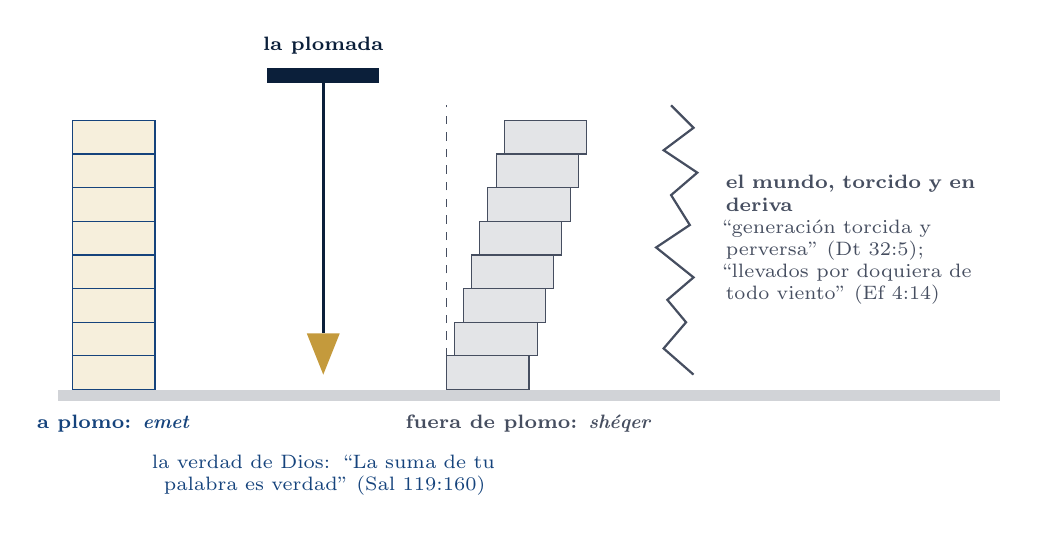
\begin{tikzpicture}[scale=0.95]
 \fill[gris!25] (-6.2,-0.15) rectangle (6.4,0);
 % muro a plomo
 \foreach \y in {0,0.45,...,3.2}{\draw[azul,fill=papiro] (-6.0,\y) rectangle (-4.9,\y+0.45);}
 \node[font=\scriptsize\bfseries,text=azul,align=center] at (-5.45,-0.45) {a plomo: \emph{emet}};
 % plomada
 \fill[azuloscuro] (-3.4,4.1) rectangle (-1.9,4.3);
 \draw[azuloscuro,line width=1pt] (-2.65,4.1) -- (-2.65,0.75);
 \fill[dorado] (-2.87,0.75) -- (-2.43,0.75) -- (-2.65,0.2) -- cycle;
 \node[font=\scriptsize\bfseries,text=azuloscuro] at (-2.65,4.6) {la plomada};
 \node[font=\scriptsize,text=azul,align=center,text width=5cm] at (-2.65,-1.15) {la verdad de Dios: ``La suma de tu palabra es verdad'' (Sal 119:160)};
 % muro torcido
 \foreach \i in {0,...,7}{\pgfmathsetmacro{\dx}{0.11*\i}\draw[gris,fill=gris!15] (-1.0+\dx,0.45*\i) rectangle (0.1+\dx,0.45*\i+0.45);}
 \draw[gris,dashed] (-1.0,0) -- (-1.0,3.8);
 \node[font=\scriptsize\bfseries,text=gris,align=center] at (0.1,-0.45) {fuera de plomo: \emph{shéqer}};
 % mundo en deriva
 \draw[gris,line width=0.8pt] (2.0,3.8) -- (2.3,3.5) -- (1.9,3.2) -- (2.35,2.9) -- (2.0,2.6) -- (2.25,2.2) -- (1.8,1.9) -- (2.3,1.5) -- (1.95,1.2) -- (2.2,0.9) -- (1.9,0.55) -- (2.3,0.2);
 \node[anchor=west,align=left,text=gris,font=\scriptsize,text width=3.6cm] at (2.6,2.0) {\textbf{el mundo, torcido y en deriva}\\ ``generación torcida y perversa'' (Dt 32:5); ``llevados por doquiera de todo viento'' (Ef 4:14)};
\end{tikzpicture}\par\medskip
{\footnotesize\color{gris}\textit{Figura 2.} La plomada: la verticalidad de la verdad. \textit{Nota.} Elaboración propia a partir del material de la serie.}
\end{center}

\subsection{La plomada en la Escritura}
La imagen de la plomada no es solo una ilustración moderna: está en los profetas.

\begin{cita}Me enseñó así: He aquí el Señor estaba sobre un muro hecho a plomo, y en su mano una plomada de albañil. \SENOR{} entonces me dijo: ¿Qué ves, Amós? Y dije: Una plomada de albañil. Y el Señor dijo: He aquí, yo pongo plomada de albañil en medio de mi pueblo Israel; no lo toleraré más.\fuente{(Am 7:7--8)}\end{cita}

\hebverso{הִנְנִי יִסַּד בְּצִיּוֹן אָבֶן אֶבֶן בֹּחַן פִּנַּת יִקְרַת מוּסָד מוּסָּד הַמַּאֲמִין לֹא יָחִישׁ \\ וְשַׂמְתִּי מִשְׁפָּט לְקָו וּצְדָקָה לְמִשְׁקָלֶת וְיָעָה בָרָד מַחְסֵה כָזָב}
\begin{cita}por tanto, \SENOR{} el Señor dice así: He aquí que yo he puesto en Sion por fundamento una piedra, piedra probada, angular, preciosa, de cimiento estable; el que creyere, no se apresure. Y ajustaré el juicio a cordel, y a nivel la justicia; y granizo barrerá el refugio de la mentira, y aguas arrollarán el escondrijo.\fuente{(Is 28:16--17)}\end{cita}

\begin{filologia}[Am 7:7--8 e Is 28:16--17]
\begin{tabular}{@{}L{3.2cm}L{1.6cm}L{10cm}@{}}
\heb{אֲנָךְ} \emph{anaj} & --- & ``plomada'' (sus cuatro apariciones están en Am 7:7--8). \\[2pt]
\heb{מִשְׁקֶלֶת} \emph{mishquélet} & \heb{שׁקל} & ``nivel, plomada'': el peso que cuelga del cordel (Is 28:17; 2~R 21:13). \\[2pt]
\heb{קַו} \emph{qav} & \heb{קוה} & ``cordel'' de medir. \\[2pt]
\heb{מוּסָד מוּסָּד} \emph{musad mussad} & \heb{יסד} & ``cimiento bien cimentado'' (RVR1960: ``de cimiento estable''). \\[2pt]
\heb{הַמַּאֲמִין} \emph{hama'amín} & \heb{אמן} & ``el que creyere'': el que se apoya en la piedra firme. \\[2pt]
\heb{מַחְסֵה כָזָב} \emph{majsé jazav} & \heb{כזב} & ``refugio de la mentira''. \\
\end{tabular}
\end{filologia}

Dios mide a su pueblo con su propia rectitud, y lo que no está a plomo cae: el ``refugio de la mentira'' lo barre el granizo. En el mismo oráculo aparece la piedra de cimiento y la raíz \emph{amán}: el que cree (\emph{hama'amín}) se apoya en lo que Dios puso firme. Pablo leerá esa piedra como Cristo (sección~\ref{sec:piedra}).

\begin{nota}[Precisión]
El sentido de \emph{anaj} se discute: HALOT propone ``estaño'' (acadio \emph{anāku}) en lugar de ``plomada''. \emph{Mishquélet}, en cambio, es con seguridad una plomada o nivel. La imagen de la plomada, por lo tanto, está firme en Is 28:17 y 2~R 21:13, y probable en Amós.
\end{nota}


\subsection{Recto y torcido}
Moisés canta la misma imagen en su último cántico. Dios es la vertical; el pueblo, lo torcido:

\hebverso{הַצּוּר תָּמִים פָּעֳלוֹ כִּי כָל־דְּרָכָיו מִשְׁפָּט אֵל אֱמוּנָה וְאֵין עָוֶל צַדִּיק וְיָשָׁר הוּא \\ שִׁחֵת לוֹ לֹא בָּנָיו מוּמָם דּוֹר עִקֵּשׁ וּפְתַלְתֹּל}
\begin{cita}El es la Roca, cuya obra es perfecta, Porque todos sus caminos son rectitud; Dios de verdad, y sin ninguna iniquidad en él; Es justo y recto. La corrupción no es suya; de sus hijos es la mancha, Generación torcida y perversa.\fuente{(Dt 32:4--5)}\end{cita}

\begin{filologia}[Dt 32:4--5]
\begin{tabular}{@{}L{3.2cm}L{1.6cm}L{10cm}@{}}
\heb{אֵל אֱמוּנָה} \emph{El emuná} & \heb{אמן} & ``Dios de verdad'': Dios de firmeza. \\[2pt]
\heb{יָשָׁר} \emph{yashar} & \heb{ישׁר} & ``recto'': derecho, a plomo. \\[2pt]
\heb{עִקֵּשׁ} \emph{iqqesh} & \heb{עקשׁ} & ``torcido'', desviado de la línea. \\[2pt]
\heb{פְּתַלְתֹּל} \emph{petaltol} & \heb{פתל} & ``retorcido'', enroscado. \\[2pt]
LXX & --- & \grc{γενεὰ σκολιὰ καὶ διεστραμμένη}, ``generación torcida y pervertida''. \\
\end{tabular}
\end{filologia}

El Predicador resume la historia humana con la misma palabra: ``Dios hizo al hombre recto (\heb{יָשָׁר}), pero ellos buscaron muchas perversiones'' (Ec 7:29). Y Pablo toma el cántico de Moisés para describir la misión de la iglesia: ``para que seáis irreprensibles y sencillos, hijos de Dios sin mancha en medio de una generación maligna y perversa (\grc{γενεᾶς σκολιᾶς καὶ διεστραμμένης}), en medio de la cual resplandecéis como luminares en el mundo'' (Flp 2:15). Los que fueron enderezados por la verdad se vuelven, en medio de lo torcido, la referencia visible.

\subsection{Todos se desviaron}
Medida con la plomada de Dios, la humanidad entera aparece fuera de la vertical:

\hebverso{הַכֹּל סָר יַחְדָּו נֶאֱלָחוּ אֵין עֹשֵׂה־טוֹב אֵין גַּם־אֶחָד}
\begin{cita}Todos se desviaron, a una se han corrompido; No hay quien haga lo bueno, no hay ni siquiera uno.\fuente{(Sal 14:3)}\end{cita}

\heb{הַכֹּל סָר}: ``todos se apartaron''; el verbo \emph{sur} es salirse del camino. Pablo cita el salmo en su diagnóstico de la humanidad: ``Todos se desviaron, a una se hicieron inútiles'' (Ro 3:12). Su verbo, \grc{ἐξέκλιναν}, es literalmente ``se inclinaron hacia afuera'': nadie quedó a plomo.

\begin{nota}[Precisión]
El material de la serie cita este salmo con otra versión (``se han vuelto inútiles'' corresponde a la forma de Ro 3:12); aquí se usa la RVR1960.
\end{nota}

\subsection{El muro que se cae de repente}
Isaías describe lo que le pasa a un muro fuera de plomo:

\hebverso{לָכֵן יִהְיֶה לָכֶם הֶעָוֹן הַזֶּה כְּפֶרֶץ נֹפֵל נִבְעֶה בְּחוֹמָה נִשְׂגָּבָה \\ אֲשֶׁר־פִּתְאֹם לְפֶתַע יָבוֹא שִׁבְרָהּ}
\begin{cita}Por tanto, el Santo de Israel dice así: Porque desechasteis esta palabra, y confiasteis en violencia y en iniquidad, y en ello os habéis apoyado; por tanto, os será este pecado como grieta que amenaza ruina, extendiéndose en una pared elevada, cuya caída viene súbita y repentinamente.\fuente{(Is 30:12--13)}\end{cita}

\begin{filologia}[Is 30:12--13]
\begin{tabular}{@{}L{3.2cm}L{1.6cm}L{10cm}@{}}
\heb{וַתִּשָּׁעֲנוּ} \emph{vatisha'anu} & \heb{שׁען} & ``y os habéis apoyado'': lo contrario de \emph{he'emín}, apoyarse en lo firme (Is 7:9). \\[2pt]
\heb{כְּפֶרֶץ נֹפֵל} \emph{keférets nofel} & \heb{פרץ} & ``como brecha que cae''. \\[2pt]
\heb{נִבְעֶה} \emph{niv'é} & \heb{בעה} & ``abombado, que sobresale'': el muro que ya se salió de la vertical. \\[2pt]
\heb{פִּתְאֹם לְפֶתַע} \emph{pitom lefeta} & --- & ``de repente, en un instante''. \\
\end{tabular}
\end{filologia}

El pecado es un muro fuera de plomo: se ve firme hasta el día en que cae, y cae de golpe. Es la misma lógica de Pr 12:19: la mentira dura ``un parpadeo''.

\subsection{Tres pasos de la plomada}
\begin{enumerate}
\item \textbf{Dios cuelga la plomada.} La medida la pone él, no nosotros: ``He aquí, yo pongo plomada de albañil en medio de mi pueblo'' (Am 7:8); ``La suma de tu palabra es verdad'' (Sal 119:160).
\item \textbf{Se mide el muro.} Las creencias, los sentimientos y las conductas se examinan contra ella: ``Examíname, oh Dios, y conoce mi corazón\ldots{} Y ve si hay en mí camino de perversidad'' (Sal 139:23--24); ``Escudriñemos nuestros caminos'' (Lam 3:40); ``Examinaos a vosotros mismos'' (2~Co 13:5).
\item \textbf{Se endereza o cae.} Lo torcido que se somete se corrige: ``Reconócelo en todos tus caminos, Y él enderezará tus veredas'' (Pr 3:6); ``lo torcido se enderece'' (Is 40:4). Lo que se resiste, cae (Is 30:13).
\end{enumerate}

\begin{cita}Fíate de \SENOR{} de todo tu corazón, Y no te apoyes en tu propia prudencia. Reconócelo en todos tus caminos, Y él enderezará tus veredas.\fuente{(Pr 3:5--6)}\end{cita}

En Pablo, la medida es una Persona. La iglesia crece ``a la medida de la estatura de la plenitud de Cristo'' (\grc{εἰς μέτρον ἡλικίας τοῦ πληρώματος τοῦ Χριστοῦ}), ``para que ya no seamos niños fluctuantes, llevados por doquiera de todo viento de doctrina\ldots{} sino que siguiendo la verdad en amor, crezcamos en todo en aquel que es la cabeza, esto es, Cristo'' (Ef 4:13--15). Cristo es la plomada; la deriva es ``todo viento de doctrina''.

%===================================================================
\section{Teología: Pink y la veracidad de Dios}

Pink no dedica un capítulo a la verdad de Dios. La trata dentro de ``La fidelidad de Dios'' (Pink, 2020, cap. 10), y esa decisión es coherente con el hebreo: \emph{emet} y \emph{emuná} vienen de la misma raíz. Se usa aquí como referencia, sin seguir su orden.

Pink comienza afirmando que la fidelidad ``es esencial para su Ser; sin ella no sería Dios. Para Dios, ser infiel, sería actuar en contra de su naturaleza, lo cual sería imposible'', y cita: ``Si fuéremos infieles, él permanece fiel; él no puede negarse a sí mismo'' (2~Ti 2:13). Luego une la fidelidad con la veracidad: ``Dios es veraz. La promesa de su Palabra es segura'' (Pink, 2020, cap. 10). Su texto central es el oráculo de Balaam:

\hebverso{לֹא אִישׁ אֵל וִיכַזֵּב וּבֶן־אָדָם וְיִתְנֶחָם}
\begin{cita}Dios no es hombre, para que mienta, Ni hijo de hombre para que se arrepienta. El dijo, ¿y no hará? Habló, ¿y no lo ejecutará?\fuente{(Nm 23:19)}\end{cita}

\begin{filologia}[Nm 23:19]
\begin{tabular}{@{}L{3.2cm}L{1.6cm}L{10cm}@{}}
\heb{וִיכַזֵּב} \emph{vijazzev} & \heb{כזב} & ``para que mienta'': el verbo de \emph{kazav}, la mentira que defrauda. \\[2pt]
\heb{וְיִתְנֶחָם} \emph{veyitnejam} & \heb{נחם} & ``para que se arrepienta'': cambie de parecer. \\
\end{tabular}
\end{filologia}

El recorrido de Pink sigue con pruebas históricas: Dios anunció a Abraham que su descendencia sería esclava y volvería ``en la cuarta generación'' (Gn 15:13--16), y ``en el mismo día'' salieron de Egipto (Éx 12:41); anunció por Isaías que la virgen concebiría (Is 7:14), y ``cuando vino el cumplimiento del tiempo, Dios envió a su Hijo'' (Gá 4:4). Pink advierte que ``una cosa es aceptar la fidelidad de Dios como una verdad divina y otra muy distinta es actuar de acuerdo con ella'', y dedica la segunda mitad del capítulo a la prueba: cuando ocurren dificultades, descansar en esta verdad silencia la queja y engendra confianza (Pink, 2020, cap. 10).

\begin{nota}[Precisión]
La fidelidad tendrá su propio estudio en esta serie (capítulo 15). Aquí se toma de Pink solo lo que toca a la veracidad de Dios.
\end{nota}

%===================================================================
\section{Las esferas de la verdad en la creación}

Si Dios es la fuente de la verdad, lo verdadero abarca todas las disciplinas humanas. Toda pregunta sobre ciencia o sobre economía política es, en el fondo, una pregunta sobre cómo Dios estructuró la realidad. Cuando la ingeniería respeta la gravedad, la estructura se mantiene en pie porque se somete a la verdad material. Jeremías 10 lo dice del Dios verdadero: es ``el que hizo la tierra con su poder, el que puso en orden el mundo con su saber, y extendió los cielos con su sabiduría'' (Jer 10:12). ``Puso en orden'' traduce \heb{מֵכִין} (\emph{mejín}), del verbo \emph{kun}, ``establecer firme''.

\subsection{La ciencia descubre}
La ciencia no inventa la verdad: la descubre. Cuando la física o las matemáticas descubren un patrón exacto en el universo, descubren la verdad del diseño de Dios. Las leyes que rigen la materia son expresiones físicas de realidades que Dios estableció. Pablo lo afirma en el comienzo de Romanos:

\begin{cita}Porque las cosas invisibles de él, su eterno poder y deidad, se hacen claramente visibles desde la creación del mundo, siendo entendidas por medio de las cosas hechas, de modo que no tienen excusa.\fuente{(Ro 1:20)}\end{cita}

El material de la serie da como ejemplo las leyes de la termodinámica.

\subsection{Primera ley: la conservación de la energía}
\textbf{El postulado.} La energía no se crea ni se destruye; solo se transforma. El universo tiene una cantidad finita de energía que cambia de estado.

\textbf{La correspondencia.} La creación de la nada es un acto exclusivo de Dios que ya concluyó: ``Y acabó Dios en el día séptimo la obra que hizo'' (Gn 2:2). El universo no puede generar nueva existencia por sí mismo. La ley ilustra también el principio bíblico del aliento de vida: cuando una persona muere, lo que la animaba no se aniquila; el cuerpo se degrada y el espíritu vuelve a su fuente.

\hebverso{וְיָשֹׁב הֶעָפָר עַל־הָאָרֶץ כְּשֶׁהָיָה וְהָרוּחַ תָּשׁוּב אֶל־הָאֱלֹהִים אֲשֶׁר נְתָנָהּ}
\begin{cita}y el polvo vuelva a la tierra, como era, y el espíritu vuelva a Dios que lo dio.\fuente{(Ec 12:7)}\end{cita}

\begin{nota}[Precisión]
La correspondencia es una analogía del material de la serie. El \emph{rúaj} (\heb{רוּחַ}, ``aliento, espíritu'') no es energía física; lo que la ley ilustra es que la creación no se crea a sí misma ni se aniquila por sí sola.
\end{nota}

\subsection{Segunda ley: la entropía}
\textbf{El postulado.} En un sistema cerrado, la energía utilizable se disipa con el tiempo y el desorden (la entropía) tiende a aumentar. Todo en el universo tiende al desgaste, al enfriamiento y a la muerte; nada se ordena a sí mismo de forma espontánea.

\textbf{La correspondencia.} El material de la serie ve aquí la demostración física de la Caída y la maldición del pecado. El universo fue creado bueno; tras la rebelión del hombre, la creación entera fue sometida a un principio de degradación y muerte. La ciencia lo llama ``aumento de entropía''; la Biblia, ``esclavitud de corrupción''.

\begin{cita}Porque la creación fue sujetada a vanidad, no por su propia voluntad, sino por causa del que la sujetó en esperanza; porque también la creación misma será libertada de la esclavitud de corrupción, a la libertad gloriosa de los hijos de Dios.\fuente{(Ro 8:20--21)}\end{cita}
\begin{cita}Desde el principio tú fundaste la tierra, Y los cielos son obra de tus manos. Ellos perecerán, mas tú permanecerás; Y todos ellos como una vestidura se envejecerán; Como un vestido los mudarás, y serán mudados; Pero tú eres el mismo, Y tus años no se acabarán.\fuente{(Sal 102:25--27 [102:26--28])}\end{cita}

\begin{filologia}[Ro 8:20--21]
\begin{tabular}{@{}L{3.2cm}L{1.6cm}L{10cm}@{}}
\grc{ματαιότης} \emph{mataiótēs} & --- & ``vanidad'': frustración, lo que no alcanza su fin. En la LXX traduce el \emph{hével} de Eclesiastés. \\[2pt]
\grc{δουλεία τῆς φθορᾶς} & --- & ``esclavitud de la corrupción'': \grc{φθορά} es descomposición, deterioro. \\
\end{tabular}
\end{filologia}

El salmista describe un universo que se gasta como ropa vieja mientras el Creador permanece; Hebreos aplica estas palabras a Cristo (He 1:10--12).

\begin{nota}[Precisión]
Identificar la segunda ley con la Caída es la lectura del material de la serie y es discutida. Otros intérpretes entienden que la segunda ley opera ya en la creación buena (el sol, por ejemplo, alumbra gastando su energía) y leen Ro 8:20 como la frustración que siguió al pecado, sin identificarla con una ley física. Lo que el texto sí afirma es que la creación actual está sometida a corrupción y espera su liberación.
\end{nota}

\subsection{Gobierno, política y economía}
En Génesis 1:28 Dios da el mandato cultural primario:

\hebverso{פְּרוּ וּרְבוּ וּמִלְאוּ אֶת־הָאָרֶץ וְכִבְשֻׁהָ וּרְדוּ}
\begin{cita}Y los bendijo Dios, y les dijo: Fructificad y multiplicaos; llenad la tierra, y sojuzgadla, y señoread en los peces del mar, en las aves de los cielos, y en todas las bestias que se mueven sobre la tierra.\fuente{(Gn 1:28)}\end{cita}

\begin{filologia}[Gn 1:28]
\begin{tabular}{@{}L{3.2cm}L{1.6cm}L{10cm}@{}}
\heb{וְכִבְשֻׁהָ} \emph{vejivshuha} & \heb{כבשׁ} & ``y sojuzgadla'': poner bajo orden lo que está sin cultivar. \\[2pt]
\heb{וּרְדוּ} \emph{uredú} & \heb{רדה} & ``y señoread'': gobernar como rey, con la autoridad delegada del Creador. \\
\end{tabular}
\end{filologia}

Lejos de ser un permiso para la explotación caprichosa, este mandato es el fundamento del orden social y material, y es anterior a la Caída (Gn 2:15). El pastor Miguel Núñez lo expresa así: ``Cada pregunta sobre política y economía es una pregunta sobre lo que significa ser hecho a la imagen de Dios y tener dominio sobre la Tierra. Dios le dijo al hombre: `sojuzga la tierra y domínala'. Bueno, para sojuzgar la tierra y dominarla habría que desarrollar algo que se llama ciencias políticas y ciencias de la economía''.

\begin{nota}[Precisión]
Esta cita de Núñez viene del material de la serie (una predicación) y falta su fuente exacta. En su libro \emph{Renueva tu mente} trata el mandato de Gn 1:28 como el fundamento del trabajo humano (Núñez, 2020, cap. 9).
\end{nota}

Bajo la plomada de la verdad, la esencia de estas disciplinas se define así:
\begin{itemize}
\item \textbf{Ciencias políticas.} No son la mera búsqueda y retención del poder, sino el diseño de sistemas de gobierno, leyes y estructuras sociales que reflejen la justicia, el orden y el carácter del Creador. Su fin es gobernar y proteger a sociedades compuestas por portadores de la imagen de Dios. Toda tiranía, corrupción o legislación que atenta contra ese diseño (como la opresión del vulnerable o la alteración de la familia) opera bajo un sistema de mentira.
\item \textbf{Economía.} Es la mayordomía fiel y eficiente de los recursos de la creación. Organiza el trabajo humano, la producción, el intercambio y la distribución de bienes para el florecimiento de la sociedad. Una economía fundada en la verdad somete el mundo material al orden divino y combate la escasez con la creatividad humana, frente a los sistemas corrompidos por la avaricia o el control opresivo.
\end{itemize}

\subsection{El fundamento de la moral}
Sin la verdad absoluta de Dios no puede existir un ser humano ni una sociedad moral. Cuando se quita la plomada, el hombre relativiza la moral a su conveniencia y se vuelve capaz de ignorar el sufrimiento ajeno. En 1996, en el Everest, un grupo de alpinistas japoneses pasó junto a escaladores que agonizaban sin ayudarlos; uno de ellos lo justificó diciendo que ``por encima de los 8000 metros no es un lugar donde la gente pueda permitirse la moralidad'' (Krakauer, 1997). Sin verdad, la moral colapsa frente a la conveniencia.

\begin{cita}Salva, oh \SENOR{}, porque se acabaron los piadosos; Porque han desaparecido los fieles de entre los hijos de los hombres. Habla mentira cada uno con su prójimo; Hablan con labios lisonjeros, y con doblez de corazón.\fuente{(Sal 12:1--2 [12:2--3])}\end{cita}

Los ``fieles'' son los \heb{אֱמוּנִים} (\emph{emunim}), los que viven en \emph{emuná}. Cuando desaparecen, desaparece la verdad entre prójimos.

\begin{nota}[Precisión]
La frase se atribuye a un miembro de la expedición japonesa de Fukuoka; conviene verificar la página en la edición del libro de Krakauer que se use.
\end{nota}

%===================================================================
\section{La verdad frente a la percepción humana}

\subsection{``Todo hombre es mentiroso''}
A causa de la Caída, el ser humano distorsiona con frecuencia la realidad para justificar sus acciones, o porque interpreta los hechos con límites.

\hebverso{אֲנִי אָמַרְתִּי בְחָפְזִי כָּל־הָאָדָם כֹּזֵב}
\begin{cita}Y dije en mi apresuramiento: Todo hombre es mentiroso.\fuente{(Sal 116:11)}\end{cita}

Pablo cita este salmo en griego y le antepone la otra mitad de la verdad:

\begin{cita}¿Pues qué, si algunos de ellos han sido incrédulos? ¿Su incredulidad habrá hecho nula la fidelidad de Dios? De ninguna manera; antes bien sea Dios veraz, y todo hombre mentiroso.\fuente{(Ro 3:3--4)}\end{cita}

\begin{center}\small\renewcommand{\arraystretch}{1.2}
\begin{tabular}{@{}L{2.6cm}L{11.8cm}@{}}
\toprule
Sal 116:11 TM & \heb{כָּל־הָאָדָם כֹּזֵב} \\
Sal 115:2 LXX & \grc{πᾶς ἄνθρωπος ψεύστης} \\
Ro 3:4 & \grc{γινέσθω δὲ ὁ θεὸς ἀληθής, πᾶς δὲ ἄνθρωπος ψεύστης} \\
\bottomrule
\end{tabular}\par
{\footnotesize\color{gris}\textit{Tabla 5.} Sal 116:11 en el texto masorético, la Septuaginta y Romanos.}
\end{center}

\subsection{Llamar a lo malo bueno}
\begin{cita}¡Ay de los que a lo malo dicen bueno, y a lo bueno malo; que hacen de la luz tinieblas, y de las tinieblas luz; que ponen lo amargo por dulce, y lo dulce por amargo!\fuente{(Is 5:20)}\end{cita}

El ``¡ay!'' (\heb{הוֹי}, \emph{hoy}) es el grito de los funerales. Cambiar el nombre de las cosas no cambia las cosas. En tiempos de Jeremías, el profeta Hananías anunció lo que el pueblo quería oír: paz en dos años (Jer 28:3). Jeremías le respondió:

\begin{cita}Entonces dijo el profeta Jeremías al profeta Hananías: Ahora oye, Hananías: \SENOR{} no te envió, y tú has hecho confiar en mentira a este pueblo.\fuente{(Jer 28:15)}\end{cita}

``Hiciste confiar'' traduce \heb{הִבְטַחְתָּ} (\emph{hivtajta}): Hananías dio al pueblo seguridad, pero una seguridad apoyada en \emph{shéqer}. La mentira cómoda se cree con facilidad; la verdad se reconoce porque se cumple (Dt 18:22; Jer 28:9, 17).

\subsection{Los sentimientos y la realidad biológica}
El material de la serie critica la idea moderna de que ``la verdad es lo que yo siento''. La verdad no se basa en los sentimientos humanos: si lo que alguien siente no corresponde con su realidad biológica o genética, ese sentimiento no es verdad. El caso más discutido hoy es la identidad sexual. El diseño genético (cromosomas XX o XY), el sistema hormonal y la estructura ósea y cerebral son marcadores de esa realidad: ``Varón y hembra los creó'' (Gn 1:27).

Núñez lo plantea en su libro sobre la cosmovisión: ``Por primera vez en la historia podemos ver que una verdad, en este caso biológica, es definida en base a un sentimiento. Algo totalmente absurdo\ldots{} Explicar la verdad tal como es, podría ayudar más a estas personas a aceptar su realidad que mutilar su cuerpo para adaptarlo a una irrealidad de la mente'' (Núñez, 2020, cap. 10). En una predicación lo dijo así: ``No es tu cuerpo el que tenemos que ajustar con cirugías, es tu mente la que tenemos que ajustar con la verdad y llevarla a la verticalidad de la verdad de Dios''.

\begin{nota}[Precisión]
La segunda cita de Núñez viene del material de la serie (una predicación) y falta su fuente exacta. La primera se cita desde la edición de 2020 de \emph{Renueva tu mente}.
\end{nota}

\subsection{Documentación clínica y legal}
Alterar la biología para acomodar una percepción genera estragos. Tres casos recientes en Estados Unidos llegaron a tribunales:

\begin{enumerate}
\item \textbf{Allan Josephson.} Psiquiatra infantil, jefe de la División de Psiquiatría y Psicología Infantil y Adolescente de la Universidad de Louisville. Fue degradado después de afirmar, en 2017, que la disforia de género en niños ``no puede abordarse plenamente con fármacos y cirugía'', y su contrato no se renovó en 2019. En 2024 el Tribunal de Apelaciones del Sexto Circuito resolvió que su demanda debía ir a juicio; en abril de 2025 la universidad acordó pagarle 1,6 millones de dólares.
\item \textbf{Fox Varian.} A los 16 años, en 2019, con un diagnóstico de autismo, recibió una mastectomía doble. El 30 de enero de 2026 un jurado de White Plains (Nueva York) condenó al psicólogo y al cirujano por mala praxis, en particular por no obtener un consentimiento informado adecuado, y le otorgó 2 millones de dólares (1,6 por daño y 0,4 por gastos médicos futuros).
\item \textbf{Kaley Chiles.} Consejera cristiana de Colorado. El 31 de marzo de 2026 la Corte Suprema de Estados Unidos resolvió, por 8 votos contra 1, que el Estado no puede aplicar su prohibición de las terapias de conversión para menores a la conversación terapéutica de Chiles, porque la ley discrimina según el punto de vista y debe pasar el escrutinio más estricto de la Primera Enmienda (\emph{Chiles v. Salazar}, 2026).
\end{enumerate}

\begin{nota}[Precisión]
Conviene presentar los casos con lo que efectivamente resolvieron. En el caso Josephson no hubo sentencia sobre el fondo: fue un acuerdo antes del juicio. En el caso Varian, el jurado juzgó el estándar de cuidado médico y el consentimiento informado. El caso Chiles es un fallo sobre libertad de expresión: la ley de Colorado prohibía a los consejeros ayudar a un menor a cambiar su orientación o identidad, y la Corte decidió que el Estado no puede silenciar uno de los lados de una cuestión moral y psicológica disputada. Fuentes: Spectrum News (21 de abril de 2025); ABA Journal (4 de febrero de 2026) y Alliance Defending Freedom; opinión de la Corte en \emph{Chiles v. Salazar}.
\end{nota}

%===================================================================
\section{Un encuentro en la historia de Israel: la viuda de Sarepta}

En tiempos de Acab, Elías anunció una sequía: ``Vive \SENOR{} Dios de Israel, en cuya presencia estoy, que no habrá lluvia ni rocío en estos años, sino por mi palabra'' (1~R 17:1). Era un desafío a Baal, el dios cananeo de la lluvia y la tormenta. Dios envió a Elías a Sarepta, en Sidón, la tierra de Jezabel; allí una viuda le dio de comer, y ``la harina de la tinaja no escaseó, ni el aceite de la vasija menguó, conforme a la palabra que \SENOR{} había dicho por Elías'' (17:16). Después murió el hijo de la viuda:

\begin{cita}Y se tendió sobre el niño tres veces, y clamó a \SENOR{} y dijo: \SENOR{} Dios mío, te ruego que hagas volver el alma de este niño a él. Y \SENOR{} oyó la voz de Elías, y el alma del niño volvió a él, y revivió. Tomando luego Elías al niño, lo trajo del aposento a la casa, y lo dio a su madre, y le dijo Elías: Mira, tu hijo vive. Entonces la mujer dijo a Elías: Ahora conozco que tú eres varón de Dios, y que la palabra de \SENOR{} es verdad en tu boca.\fuente{(1~R 17:21--24)}\end{cita}

\hebverso{עַתָּה זֶה יָדַעְתִּי כִּי אִישׁ אֱלֹהִים אָתָּה וּדְבַר־יְהוָה בְּפִיךָ אֱמֶת}

\begin{filologia}[1 R 17:24]
\begin{tabular}{@{}L{3.2cm}L{1.6cm}L{10cm}@{}}
\heb{עַתָּה זֶה יָדַעְתִּי} \emph{attá ze yadati} & \heb{ידע} & ``ahora sí sé'': un conocimiento nuevo, por experiencia. \\[2pt]
\heb{וּדְבַר־יְהוָה בְּפִיךָ אֱמֶת} & \heb{אמן} & ``y la palabra del \SENOR{} en tu boca es \emph{emet}'': firme, confiable, verdadera. \\[2pt]
\heb{רְאִי חַי בְּנֵךְ} \emph{re'í jay benej} & \heb{חיה} & ``mira, tu hijo vive'' (17:23). \\
\end{tabular}
\end{filologia}

La mujer ya llamaba a Elías ``varón de Dios'' (17:18). Ahora \emph{conoce}: la palabra es \emph{emet} porque devolvió la vida. En la tierra de Baal, el dios que no pudo dar lluvia, el \SENOR{} devolvió un hijo. El relato prepara la confesión del Carmelo: ``¡\SENOR{} es el Dios, \SENOR{} es el Dios!'' (1~R 18:39). Es el mismo contraste de Jer 10:10: el Dios verdadero es el Dios vivo.

Jesús recuerda a esta viuda en la sinagoga de Nazaret: ``muchas viudas había en Israel en los días de Elías\ldots{} pero a ninguna de ellas fue enviado Elías, sino a una mujer viuda en Sarepta de Sidón'' (Lc 4:25--26). En Naín resucita al hijo único de otra viuda, y Lucas narra el final con las mismas palabras de la Septuaginta: \grc{καὶ ἔδωκεν αὐτὸν τῇ μητρὶ αὐτοῦ}, ``y lo dio a su madre'' (Lc 7:15 = 1~R 17:23 LXX).

\begin{nota}[Precisión]
El eco verbal entre 1~R 17:23 (LXX) y Lc 7:15 está en el texto griego. La conexión entre la confesión de la viuda y Jer 10:10 es una lectura propia de esta serie.
\end{nota}

%===================================================================
\section{La verdad en el judaísmo}

\subsection{``El sello del Santo es \emph{emet}''}
El Talmud de Babilonia, al comentar la marca que el ángel pone en la frente de los justos en Ezequiel 9, cita a Rabí Janiná:

\hebverso{חוֹתָמוֹ שֶׁל הַקָּדוֹשׁ בָּרוּךְ הוּא אֱמֶת}

``El sello del Santo, bendito sea, es \emph{emet}'' (\emph{Shabat} 55a). El Talmud de Jerusalén conserva la misma tradición y la explica (\emph{Sanedrín} 1:1). Ante la pregunta ``¿qué es el sello del Santo?'', responde ``\emph{emet}''; Rabí Bun explica qué significa: \heb{שֶׁהוּא אֱלֹהִים חַיִּים וּמֶלֶךְ עוֹלָם}, ``que él es Dios vivo y Rey eterno'', las palabras de Jer 10:10. Y Resh Laquish observa que álef es la primera letra del alfabeto, mem la del medio y tav la última: Dios es el primero, que no recibió de otro, y el último, que no entregará a otro (Is 41:4; cf. 44:6).

\begin{nota}[Precisión]
Interpretación rabínica. Texto según Sefaria (Talmud de Babilonia, edición William Davidson; Talmud de Jerusalén, edición de Guggenheimer). La lectura de las tres letras es un juego interpretativo, no una etimología.
\end{nota}

\subsection{La verdad tiene pies anchos}
En otra página, el Talmud compara las palabras \emph{shéqer} (\heb{שקר}) y \emph{emet} (\heb{אמת}). Las letras de \emph{shéqer} están juntas en el alfabeto (\heb{ש ק ר}); las de \emph{emet}, separadas: la mentira es común, la verdad escasa. Además, las letras de \emph{shéqer} se apoyan sobre un solo punto; las de \emph{emet}, sobre una base ancha:

\hebverso{קוּשְׁטָא קָאֵי שִׁיקְרָא לָא קָאֵי}

``La verdad se mantiene en pie; la mentira no se mantiene'' (\emph{Shabat} 104a). Es la plomada del material de la serie dicha por los sabios, y la misma idea de Pr 12:19.

\begin{nota}[Precisión]
Interpretación rabínica sobre la forma de las letras hebreas cuadradas, según Sefaria.
\end{nota}

\subsection{La verdad arrojada a la tierra}
El midrash \emph{Bereshit Rabá} (8:5) cuenta, en nombre de Rabí Simón, que cuando Dios iba a crear al hombre los ángeles se dividieron. La Misericordia dijo: ``que sea creado'', porque hará actos de bondad; la Verdad dijo: ``que no sea creado'', \heb{שֶׁכֻּלּוֹ שְׁקָרִים}, ``porque todo él es mentiras''. La Justicia y la Paz también discutieron. ¿Qué hizo el Santo? \heb{נָטַל אֱמֶת וְהִשְׁלִיכוֹ לָאָרֶץ}, ``tomó la verdad y la arrojó a la tierra'', como dice Dn 8:12 (``echó por tierra la verdad''). Y los sabios cierran con el Salmo:

\hebverso{אֱמֶת מֵאֶרֶץ תִּצְמָח וְצֶדֶק מִשָּׁמַיִם נִשְׁקָף}
\begin{cita}La misericordia y la verdad se encontraron; La justicia y la paz se besaron. La verdad brotará de la tierra, Y la justicia mirará desde los cielos.\fuente{(Sal 85:10--11 [85:11--12])}\end{cita}

\begin{nota}[Precisión]
Interpretación rabínica (midrash). La lectura cristiana que ve en Cristo ``la verdad que brota de la tierra'' (cf. Jn 1:14) no pertenece al midrash.
\end{nota}

\subsection{La verdad en la oración y en la Misná}
\begin{itemize}
\item \textbf{Después del \emph{Shemá}.} El \emph{Shemá} termina con ``Yo soy el \SENOR{} vuestro Dios'' (Nm 15:41). El Talmud enseña que en seguida se dice \emph{emet}, ``verdad'', y lo apoya en Jer 10:10: \heb{וַיהוָה אֱלֹהִים אֱמֶת} (\emph{Berajot} 14b). En la oración diaria el Nombre y la verdad no se separan.
\item \textbf{\emph{Emet veyatsiv}.} La bendición de la mañana que sigue al \emph{Shemá} comienza \heb{אֱמֶת וְיַצִּיב}, ``verdadero y firme'', y la de la tarde \heb{אֱמֶת וֶאֱמוּנָה}, ``verdad y fidelidad'' (Elbogen, 1993).
\item \textbf{\emph{Avot} 1:18.} Rabán Shimón ben Gamliel: \heb{עַל שְׁלֹשָׁה דְבָרִים הָעוֹלָם עוֹמֵד}, ``sobre tres cosas se sostiene el mundo: la justicia, la verdad y la paz'', y cita Zac 8:16.
\item \textbf{Maimónides.} En el primer capítulo de la \emph{Mishné Torá} (\emph{Yesodé haTorá} 1:4) cita Jer 10:10 y comenta: \heb{הוּא לְבַדּוֹ הָאֱמֶת וְאֵין לְאַחֵר אֱמֶת כַּאֲמִתָּתוֹ}, ``él solo es la verdad, y ningún otro tiene verdad como la suya''.
\end{itemize}

\begin{cita}Estas son las cosas que habéis de hacer: Hablad verdad cada cual con su prójimo; juzgad según la verdad y lo conducente a la paz en vuestras puertas.\fuente{(Zac 8:16)}\end{cita}

\begin{nota}[Precisión]
Interpretaciones y usos litúrgicos judíos, según Sefaria. Tres de las cuatro fuentes se apoyan en el texto ancla de este capítulo, Jer 10:10.
\end{nota}

\subsection{Qumrán: el espíritu de verdad}
La \emph{Regla de la Comunidad} de Qumrán (1QS) enseña que Dios puso en el hombre dos espíritus para andar en ellos hasta el tiempo de su visitación: \heb{רוּחוֹת הָאֱמֶת וְהָעָוֶל}, ``los espíritus de la verdad y de la perversidad'' (1QS 3:18--19). ``Los nacidos de la verdad brotan de una fuente de luz, y los nacidos de la perversidad, de un manantial de tinieblas'' (1QS 3:19). Al final, Dios ``rociará sobre él el espíritu de verdad como aguas de purificación'' (1QS 4:21), un lenguaje que recuerda Ez 36:25--27. Y quien entra en la comunidad se compromete ``a practicar la verdad, la justicia y el derecho en la tierra'' (1QS 1:5), un eco de Jer 9:24.

El Evangelio de Juan usa un vocabulario cercano: ``el Espíritu de verdad, al cual el mundo no puede recibir'' (Jn 14:17) y ``el que practica la verdad viene a la luz'' (Jn 3:21).

\begin{nota}[Precisión]
Traducción según García Martínez (1992) y Vermes (2004); conviene cotejar las imágenes de 1QS en la Leon Levy Dead Sea Scrolls Digital Library. Los paralelos con Juan los señalan los estudios del Nuevo Testamento; muestran un lenguaje judío común, no una dependencia directa. Sobre Qumrán y el texto de Jeremías 10, véase la precisión textual sobre Jeremías 10 en la sección~\ref{sec:jer10}.
\end{nota}

%===================================================================
\section{La verdad en Cristo, leída con Pablo}

\subsection{Cambiaron la verdad por la mentira}
Pablo comienza su exposición del evangelio con el mismo diagnóstico de Jeremías 10:

\begin{cita}Porque la ira de Dios se revela desde el cielo contra toda impiedad e injusticia de los hombres que detienen con injusticia la verdad\ldots{} ya que cambiaron la verdad de Dios por la mentira, honrando y dando culto a las criaturas antes que al Creador, el cual es bendito por los siglos. Amén.\fuente{(Ro 1:18, 25)}\end{cita}

\begin{filologia}[Ro 1:18, 25]
\begin{tabular}{@{}L{3.2cm}L{1.6cm}L{10cm}@{}}
\grc{τὴν ἀλήθειαν\ldots{} κατεχόντων} & \grc{κατέχω} & ``que sujetan, retienen la verdad'': la verdad está a la vista, pero la reprimen. \\[2pt]
\grc{μετήλλαξαν} \emph{metéllaxan} & \grc{ἀλλάσσω} & ``trocaron'': cambiaron una cosa por otra. \\[2pt]
\grc{ἐν τῷ ψεύδει} & \grc{ψεῦδος} & ``por \emph{la} mentira'', con artículo: el ídolo. La LXX de Jer 10:14 dice de los fundidores \grc{ψευδῆ ἐχώνευσαν}, ``fundieron mentiras''. \\[2pt]
\grc{ἀμήν} & --- & Pablo cierra la denuncia con un ``Amén'': frente a la mentira, la confesión de lo firme. \\
\end{tabular}
\end{filologia}

Para Pablo, ``la mentira'' es primero el ídolo, como para Jeremías. La verdad de Dios es Dios mismo, conocido por medio de lo creado (Ro 1:20) y cambiado por una imagen.

\begin{nota}[Precisión]
Leer ``la mentira'' de Ro 1:25 como la idolatría es común entre los comentaristas (Moo, 1996); el vínculo con Jer 10:14 es una lectura propia de esta serie.
\end{nota}

\subsection{``Sea Dios veraz''}
En Romanos 3 Pablo enfrenta una objeción: si Israel fue infiel, ¿no queda anulada la fidelidad de Dios?

\begin{cita}¿Pues qué, si algunos de ellos han sido incrédulos? ¿Su incredulidad habrá hecho nula la fidelidad de Dios? De ninguna manera; antes bien sea Dios veraz, y todo hombre mentiroso; como está escrito: Para que seas justificado en tus palabras, Y venzas cuando fueres juzgado.\fuente{(Ro 3:3--4)}\end{cita}

Pablo une las dos caras de la raíz \emph{amán}. La ``incredulidad'' (\grc{ἀπιστία}) de algunos no anula ``la fidelidad de Dios'' (\grc{τὴν πίστιν τοῦ θεοῦ}); Dios es ``veraz'' (\grc{ἀληθής}) porque cumple lo que prometió aunque Israel falle. En 3:7 llama a lo mismo ``la verdad de Dios'' (\grc{ἡ ἀλήθεια τοῦ θεοῦ}). Es Nm 23:19 leído en Romanos: Dios no es hombre para que mienta.

\subsection{Cristo, siervo de la verdad de Dios}
\begin{cita}Pues os digo, que Cristo Jesús vino a ser siervo de la circuncisión para mostrar la verdad de Dios, para confirmar las promesas hechas a los padres, y para que los gentiles glorifiquen a Dios por su misericordia.\fuente{(Ro 15:8--9)}\end{cita}

\begin{filologia}[Ro 15:8]
\begin{tabular}{@{}L{3.2cm}L{1.6cm}L{10cm}@{}}
\grc{ὑπὲρ ἀληθείας θεοῦ} & \grc{ἀλήθεια} & ``a favor de la verdad de Dios'': para mostrar que Dios es fiel. \\[2pt]
\grc{εἰς τὸ βεβαιῶσαι} & \grc{βεβαιόω} & ``para confirmar, hacer firmes'' las promesas: casi una traducción de \emph{amán}. \\
\end{tabular}
\end{filologia}

Miqueas había pedido: ``Cumplirás la verdad a Jacob, y a Abraham la misericordia, que juraste a nuestros padres desde tiempos antiguos'' (Mi 7:20). Pablo dice que Cristo trajo la verdad (\emph{emet}) a Israel y la misericordia (\emph{jésed}) a las naciones. Jesús es la prueba histórica de que Dios es \emph{Elohim emet}.

\subsection{``En él Sí, y en él Amén''}
\begin{cita}Mas, como Dios es fiel, nuestra palabra a vosotros no es Sí y No. Porque el Hijo de Dios, Jesucristo, que entre vosotros ha sido predicado por nosotros, por mí, Silvano y Timoteo, no ha sido Sí y No; mas ha sido Sí en él; porque todas las promesas de Dios son en él Sí, y en él Amén, por medio de nosotros, para la gloria de Dios.\fuente{(2~Co 1:18--20)}\end{cita}

\grc{ὅσαι γὰρ ἐπαγγελίαι θεοῦ, ἐν αὐτῷ τὸ ναί· διὸ καὶ δι᾽ αὐτοῦ τὸ ἀμήν}. El ``Sí'' es la respuesta de Dios a sus propias promesas en Cristo; el ``Amén'' es la respuesta de la iglesia, que lo confiesa ``para la gloria de Dios''. Isaías había llamado a Dios \emph{Elohé amén} (Is 65:16); el Apocalipsis llama a Cristo ``el Amén, el testigo fiel y verdadero'' (Ap 3:14).

\begin{center}
\begin{tikzpicture}[font=\small,node distance=0.9cm]
 \node[draw=azul,line width=0.8pt,fill=papiro,rounded corners=3pt,text width=3.4cm,align=center,inner sep=6pt] (a) {\textbf{Is 65:16}\\ \heb{אֱלֹהֵי אָמֵן}\\ ``el Dios del Amén''};
 \node[draw=azul,line width=0.8pt,fill=papiro,rounded corners=3pt,text width=3.4cm,align=center,inner sep=6pt,right=of a] (b) {\textbf{2 Co 1:20}\\ \grc{δι᾽ αὐτοῦ τὸ ἀμήν}\\ ``en él Amén''};
 \node[draw=dorado,line width=1.6pt,fill=azul,text=papiro,rounded corners=3pt,text width=3.4cm,align=center,inner sep=6pt,right=of b] (c) {\textbf{Ap 3:14}\\ \grc{ὁ ἀμήν}\\ ``el Amén, el testigo fiel y verdadero''};
 \draw[-{Latex[length=3mm]},dorado,line width=1.4pt] (a)--(b);
 \draw[-{Latex[length=3mm]},dorado,line width=1.4pt] (b)--(c);
\end{tikzpicture}\par
{\footnotesize\color{gris}\textit{Figura 3.} Del Dios del Amén al Amén encarnado. \textit{Nota.} Elaboración propia.}
\end{center}

\subsection{El Dios vivo y verdadero}
\begin{cita}porque ellos mismos cuentan de nosotros la manera en que nos recibisteis, y cómo os convertisteis de los ídolos a Dios, para servir al Dios vivo y verdadero, y esperar de los cielos a su Hijo, al cual resucitó de los muertos, a Jesús, quien nos libra de la ira venidera.\fuente{(1~Ts 1:9--10)}\end{cita}

Primera Tesalonicenses es probablemente la carta más antigua de Pablo. Al resumir su predicación a gentiles usa el lenguaje de Jeremías 10: dejar los ídolos para servir \grc{θεῷ ζῶντι καὶ ἀληθινῷ}, ``al Dios vivo y verdadero'' (cf. \heb{אֱלֹהִים אֱמֶת}\ldots{} \heb{אֱלֹהִים חַיִּים}, Jer 10:10). Y la prueba de que Dios está vivo es que resucitó a su Hijo, lo que en Sarepta fue un anticipo.

\begin{nota}[Precisión]
Jer 10:10 falta en la Septuaginta. Pablo usa una fórmula judía corriente (cf. Is 65:16 LXX, \grc{τὸν θεὸν τὸν ἀληθινόν}); el eco de Jeremías 10 es probable, no seguro.
\end{nota}

\subsection{La verdad está en Jesús}
El Antiguo Testamento preparó a Israel revelando a un Dios que es firme y exige firmeza. La revelación culminante del Nuevo Testamento es que la verdad no es un simple concepto ni una idea filosófica: es una Persona.

\begin{cita}Mas vosotros no habéis aprendido así a Cristo, si en verdad le habéis oído, y habéis sido por él enseñados, conforme a la verdad que está en Jesús.\fuente{(Ef 4:20--21)}\end{cita}

``Conforme a la verdad que está en Jesús'' (\grc{καθώς ἐστιν ἀλήθεια ἐν τῷ Ἰησοῦ}). Juan lo dice con palabras de Éxodo 34:6 (\emph{rav jésed ve'emet}): el Verbo ``fue hecho carne\ldots{} lleno de gracia y de verdad'' (Jn 1:14); ``la ley por medio de Moisés fue dada, pero la gracia y la verdad vinieron por medio de Jesucristo'' (Jn 1:17). Y Jesús lo dice de sí mismo:

\begin{cita}Jesús le dijo: Yo soy el camino, y la verdad, y la vida; nadie viene al Padre, sino por mí.\fuente{(Jn 14:6)}\end{cita}

Cuando Jesucristo declara ``Yo soy\ldots{} la verdad'', habla de su propia naturaleza encarnada. Por eso Pablo advierte: ``Mirad que nadie os engañe por medio de filosofías y huecas sutilezas\ldots{} y no según Cristo. Porque en él habita corporalmente toda la plenitud de la Deidad'' (Col 2:8--9). Lo que no está a plomo con Cristo no está a plomo con la realidad.

\begin{nota}[Precisión]
Juan no es Pablo; se cita porque Pablo dice lo mismo con otras palabras. La autoría de Efesios y Colosenses se discute; Ro 15:8 y 2~Co 1:20 afirman lo mismo en cartas indiscutidas.
\end{nota}

\subsection{La piedra de cimiento estable}\label{sec:piedra}
En Isaías 28, Dios pone en Sion una piedra probada y mide con cordel y plomada; el que cree (\emph{hama'amín}) no queda en vergüenza. Pablo cita ese oráculo dos veces y lo aplica a Cristo:

\begin{cita}como está escrito: He aquí pongo en Sion piedra de tropiezo y roca de caída; Y el que creyere en él, no será avergonzado.\fuente{(Ro 9:33)}\end{cita}
\begin{cita}Pues la Escritura dice: Todo aquel que en él creyere, no será avergonzado.\fuente{(Ro 10:11)}\end{cita}

\begin{center}\small\renewcommand{\arraystretch}{1.2}
\begin{tabular}{@{}L{2.4cm}L{12.0cm}@{}}
\toprule
Is 28:16 TM & \heb{מוּסָד מוּסָּד הַמַּאֲמִין לֹא יָחִישׁ}: ``cimiento bien cimentado; el que cree no se apresurará'' \\
Is 28:16 LXX & \grc{ὁ πιστεύων ἐπ᾽ αὐτῷ οὐ μὴ καταισχυνθῇ}: ``el que cree en él no será avergonzado'' \\
Ro 10:11 & \grc{πᾶς ὁ πιστεύων ἐπ᾽ αὐτῷ οὐ καταισχυνθήσεται}: Pablo agrega ``todo aquel'' \\
\bottomrule
\end{tabular}\par
{\footnotesize\color{gris}\textit{Tabla 6.} Is 28:16 en el TM, la LXX y Romanos.}
\end{center}

La cadena es completa: \emph{amán} es sostener; \emph{emet} es lo que sostiene; \emph{he'emín} es apoyarse en ello; y Cristo es la piedra firme en que se apoya el que cree.

\subsection{Mentir profana a una Persona}
Las implicaciones son eternas. Cuando alguien miente o se alía con la falsedad, no deshonra solo un concepto ético abstracto: profana a una Persona, a Jesús, y se alía con el padre de mentira.

\begin{cita}Vosotros sois de vuestro padre el diablo, y los deseos de vuestro padre queréis hacer. El ha sido homicida desde el principio, y no ha permanecido en la verdad, porque no hay verdad en él. Cuando habla mentira, de suyo habla; porque es mentiroso, y padre de mentira.\fuente{(Jn 8:44)}\end{cita}

Pablo saca la consecuencia para la iglesia:

\begin{cita}Por lo cual, desechando la mentira, hablad verdad cada uno con su prójimo; porque somos miembros los unos de los otros.\fuente{(Ef 4:25)}\end{cita}

\grc{λαλεῖτε ἀλήθειαν ἕκαστος μετὰ τοῦ πλησίον αὐτοῦ} es casi palabra por palabra Zac 8:16 en la Septuaginta (\grc{λαλεῖτε ἀλήθειαν ἕκαστος πρὸς τὸν πλησίον αὐτοῦ}). La razón es nueva: ``somos miembros los unos de los otros''. Mentir al hermano es mentir dentro del cuerpo de Cristo.

\subsection{La verdad que hace libres}
\begin{cita}Si vosotros permaneciereis en mi palabra, seréis verdaderamente mis discípulos; y conoceréis la verdad, y la verdad os hará libres.\fuente{(Jn 8:31--32)}\end{cita}

La libertad viene de \emph{permanecer} (\grc{μένω}) en su palabra: otra vez la firmeza. Pablo describe su ministerio como ``manifestación de la verdad'' y lo funda en la gloria vista en Cristo: ``Dios, que mandó que de las tinieblas resplandeciese la luz, es el que resplandeció en nuestros corazones, para iluminación del conocimiento de la gloria de Dios en la faz de Jesucristo'' (2~Co 4:2, 6). Solo sujetos a Cristo, la Verdad encarnada y la plomada absoluta del universo, encontramos salvación y libertad.

%===================================================================
\section{Aplicación: un atributo comunicable}

\subsection{Hablar verdad en el corazón}
\hebverso{הוֹלֵךְ תָּמִים וּפֹעֵל צֶדֶק וְדֹבֵר אֱמֶת בִּלְבָבוֹ}
\begin{cita}\SENOR{}, ¿quién habitará en tu tabernáculo? ¿Quién morará en tu monte santo? El que anda en integridad y hace justicia, Y habla verdad en su corazón.\fuente{(Sal 15:1--2)}\end{cita}

``Habla verdad \emph{en} su corazón'' (\heb{בִּלְבָבוֹ}): la verdad empieza adentro, antes de llegar a los labios. ``He aquí, tú amas la verdad en lo íntimo'' (Sal 51:6 [51:8]). Como fuente, la verdad es solo de Dios; como veracidad, se comunica a quien vive delante de él.

\subsection{Siguiendo la verdad en amor}
Pablo pide a la iglesia que crezca ``siguiendo la verdad en amor'' (\grc{ἀληθεύοντες δὲ ἐν ἀγάπῃ}, Ef 4:15). El verbo \grc{ἀληθεύω} es ``decir la verdad, vivir en la verdad''. Verdad sin amor hiere; amor sin verdad engaña. Zacarías lo había dicho como un mandato para el tiempo de la restauración: ``Amad, pues, la verdad y la paz'' (\heb{וְהָאֱמֶת וְהַשָּׁלוֹם אֱהָבוּ}, Zac 8:19).

\subsection{Cuatro respuestas}
\begin{enumerate}
\item \textbf{Dejar los ídolos.} Servir al Dios vivo y verdadero, no a lo que fabricamos y clavamos para que no se caiga (Jer 10:4, 10; 1~Ts 1:9).
\item \textbf{Ajustarse a la plomada.} Dejar que la Palabra mida la mente y los sentimientos: ``Santifícalos en tu verdad; tu palabra es verdad'' (Jn 17:17); ``transformaos por medio de la renovación de vuestro entendimiento'' (Ro 12:2).
\item \textbf{Hablar verdad.} Con el prójimo, en amor, porque somos un cuerpo (Ef 4:15, 25; Zac 8:16).
\item \textbf{Amar la verdad.} Recibir ``el amor de la verdad'' y no la mentira cómoda (2~Ts 2:10; Zac 8:19).
\end{enumerate}

\begin{cita}y con todo engaño de iniquidad para los que se pierden, por cuanto no recibieron el amor de la verdad para ser salvos.\fuente{(2~Ts 2:10)}\end{cita}

La pregunta que deja el material de la serie es personal: ¿estoy dispuesto a ajustar mi mente, mis emociones y mi vida a la plomada de la verdad de Dios, o espero que la verdad se incline a lo que yo siento?

%===================================================================
\section{Síntesis}

\begin{tcolorbox}[colback=papiro,colframe=azul,boxrule=1pt,arc=3pt]
Frente a ídolos clavados para no caerse, Jeremías confiesa: ``Mas \SENOR{} es el Dios verdadero'' (\emph{Elohim emet}, Jer 10:10). La verdad de Dios es firmeza (raíz \emph{amán}), correspondencia con la realidad que él creó y fidelidad a lo que promete. Es la plomada de la ciencia, la política y la moral, y juzga lo que sentimos. Israel la llamó el ``sello'' de Dios; Pablo la vio confirmada en Cristo, en quien todas las promesas son ``Sí'' y ``Amén'' (2~Co 1:20).
\end{tcolorbox}

\begin{center}\small\renewcommand{\arraystretch}{1.3}
\begin{tabular}{@{}L{3.0cm}L{11.4cm}@{}}
\toprule
\textbf{Mirada} & \textbf{Aporte al atributo} \\ \midrule
Hebrea & \emph{emet}, \emph{emuná}, \emph{amén}; Jeremías 10 (el Dios vivo frente al ídolo \emph{shéqer}); la plomada (Am 7; Is 28); Pr 12:19; la viuda de Sarepta. \\
Judía & El sello de Dios es \emph{emet}; \emph{shéqer} sobre un pie; \emph{emet} después del \emph{Shemá}; \emph{Avot} 1:18; Maimónides; el espíritu de verdad en 1QS. \\
Pink & La veracidad dentro de la fidelidad: esencial a su ser, probada en la historia, para vivirla en la prueba. \\
Paulina & Ro 1:25; 3:4; 15:8; 2~Co 1:20; 1~Ts 1:9; Ef 4:21, 25; Cristo, la piedra firme (Ro 9:33; 10:11). \\
\bottomrule
\end{tabular}\end{center}

\begin{cita}Mas alábese en esto el que se hubiere de alabar: en entenderme y conocerme, que yo soy \SENOR{}, que hago misericordia, juicio y justicia en la tierra; porque estas cosas quiero, dice \SENOR{}.\fuente{(Jer 9:24 [9:23])}\end{cita}

El verso que une esta obra pide conocer a Dios; el capítulo siguiente de Jeremías dice quién es: el Dios verdadero, vivo y Rey eterno. Conocerlo es apoyarse en lo único que no se cae.

%===================================================================
\section*{Compendio bíblico}
\begin{center}\small\renewcommand{\arraystretch}{1.12}
\begin{tabular}{@{}L{2.2cm}L{5.0cm}|L{2.2cm}L{5.0cm}@{}}
\toprule
Gn 1:28 & ``llenad la tierra, y sojuzgadla'' & Jn 1:14 & ``lleno de gracia y de verdad'' \\
Sal 15:1--2 & ``Y habla verdad en su corazón'' & Jn 3:21 & ``el que practica la verdad viene a la luz'' \\
Sal 26:3 & ``Y ando en tu verdad'' & Jn 4:23--24 & ``en espíritu y en verdad'' \\
Sal 31:5 & ``oh \SENOR{}, Dios de verdad'' & Jn 8:32 & ``la verdad os hará libres'' \\
Sal 43:3 & ``Envía tu luz y tu verdad'' & Jn 8:44 & ``es mentiroso, y padre de mentira'' \\
Sal 58:3 & ``hablando mentira desde que nacieron'' & Jn 14:6 & ``Yo soy el camino, y la verdad'' \\
Sal 86:11 & ``caminaré yo en tu verdad'' & Jn 14:17; 15:26 & ``el Espíritu de verdad'' \\
Sal 116:11 & ``Todo hombre es mentiroso'' & Jn 16:13 & ``os guiará a toda la verdad'' \\
Sal 119:30 & ``Escogí el camino de la verdad'' & Ro 1:25 & ``cambiaron la verdad de Dios por la mentira'' \\
Sal 119:89 & ``Permanece tu palabra en los cielos'' & 1~Co 3:18 & ``Nadie se engañe a sí mismo'' \\
Sal 119:160 & ``La suma de tu palabra es verdad'' & 2~Co 1:20 & ``en él Sí, y en él Amén'' \\
Pr 6:16--19 & ``la lengua mentirosa\ldots{} El testigo falso'' & Gá 6:7 & ``Dios no puede ser burlado'' \\
Pr 19:5 & ``el que habla mentiras no escapará'' & Ef 5:6 & ``Nadie os engañe con palabras vanas'' \\
Ec 12:7 & ``el espíritu vuelva a Dios que lo dio'' & Col 2:8 & ``nadie os engañe por medio de filosofías'' \\
Sal 102:25--26 & ``como una vestidura se envejecerán'' & 2~Ti 2:15 & ``que usa bien la palabra de verdad'' \\
Is 5:20 & ``a lo malo dicen bueno'' & He 6:18 & ``es imposible que Dios mienta'' \\
Is 65:16 & ``en el Dios de verdad se bendecirá'' & Stg 1:16 & ``Amados hermanos míos, no erréis'' \\
Jer 5:1 & ``si hay alguno\ldots{} que busque verdad'' & 1~P 1:22 & ``por la obediencia a la verdad'' \\
Jer 10:10 & ``Mas \SENOR{} es el Dios verdadero'' & 1~Jn 1:8; 3:7 & ``la verdad no está en nosotros''; ``nadie os engañe'' \\
Zac 8:19 & ``Amad, pues, la verdad y la paz'' & 3~Jn 3, 8 & ``tu verdad''; ``cooperemos con la verdad'' \\
 & & Ap 16:7; 19:2 & ``tus juicios son verdaderos y justos'' \\
 & & Ap 19:9, 11 & ``palabras verdaderas''; ``Fiel y Verdadero'' \\
\bottomrule
\end{tabular}\par
{\footnotesize\color{gris}\textit{Tabla 7.} Compendio bíblico de la verdad. \textit{Nota.} Textos del material de la serie más el texto ancla, en la RVR1960.}
\end{center}

%===================================================================
\section*{Glosario}
\begin{description}\setlength{\itemsep}{2pt}
\item[\emph{Alétheia}] (\grc{ἀλήθεια}). Verdad; en la LXX traduce \emph{emet}.
\item[\emph{Alēthinós}] (\grc{ἀληθινός}). Genuino, verdadero, real (1~Ts 1:9; Jn 15:1).
\item[\emph{Amán}] (\heb{אָמַן}). Sostener, cargar; ser firme; en hifil, creer.
\item[\emph{Amén}] (\heb{אָמֵן}, \grc{ἀμήν}). ``Así es'', ``firme''; ``el Dios del Amén'' (Is 65:16); ``el Amén'' (Ap 3:14).
\item[\emph{Anaj}] (\heb{אֲנָךְ}). Plomada (o estaño) (Am 7:7--8).
\item[\emph{Apseudés}] (\grc{ἀψευδής}). Que no miente (Tit 1:2).
\item[\emph{Elohim emet}] (\heb{אֱלֹהִים אֱמֶת}). ``Dios verdad'' (Jer 10:10).
\item[\emph{Dípsijos}] (\grc{δίψυχος}). ``De doble alma'', con doblez (Stg 1:8).
\item[\emph{Emet}] (\heb{אֱמֶת}). Verdad, firmeza, fidelidad.
\item[\emph{Emet veyatsiv}] (\heb{אֱמֶת וְיַצִּיב}). ``Verdadero y firme'': bendición matinal después del \emph{Shemá}.
\item[\emph{Emuná}] (\heb{אֱמוּנָה}). Fidelidad, firmeza; fe.
\item[\emph{He'emín}] (\heb{הֶאֱמִין}). Creer: apoyarse en lo firme (Is 7:9).
\item[\emph{Hével}] (\heb{הֶבֶל}). Vanidad, vapor (Jer 10:3).
\item[\emph{Iqqesh}] (\heb{עִקֵּשׁ}). Torcido, desviado (Dt 32:5).
\item[\emph{Jotam}] (\heb{חוֹתָם}). Sello: ``el sello del Santo es \emph{emet}''.
\item[\emph{Kazav}] (\heb{כָּזָב}). Mentira; el verbo: mentir (Sal 116:11; Nm 23:19).
\item[\emph{Mishquélet}] (\heb{מִשְׁקֶלֶת}). Nivel, plomada (Is 28:17; 2~R 21:13).
\item[\emph{Ne'emán}] (\heb{נֶאֱמָן}). Firme, fiel, estable.
\item[\emph{Omnam}] (\heb{אָמְנָם}). Verdaderamente.
\item[\emph{Phōs}] (\grc{φῶς}). Luz: ``Dios es luz'' (1~Jn 1:5).
\item[\emph{Pseûdos}] (\grc{ψεῦδος}). Mentira (Ro 1:25; Ef 4:25).
\item[\emph{Qeshot}] (arameo \heb{קְשֹׁט}). Verdad (Dn 4:37).
\item[\emph{Shéqer}] (\heb{שֶׁקֶר}). Mentira, falsedad, engaño (Jer 10:14).
\item[\emph{Yashar}] (\heb{יָשָׁר}). Recto, derecho, a plomo (Dt 32:4; Ec 7:29).
\end{description}

\section*{Referencias}
\refapa{\emph{Bereshit Rabá} [8:5]. (s.f.). Sefaria. https://www.sefaria.org}
\refapa{Carson, D.~A. (2013). \emph{Falacias exegéticas}. Editorial CLIE.}
\refapa{\emph{Chiles v. Salazar}, No. 24-539 (Corte Suprema de EE.~UU., 31 de marzo de 2026).}
\refapa{Elbogen, I. (1993). \emph{Jewish liturgy: A comprehensive history} (R.~P. Scheindlin, Trad.). Jewish Publication Society.}
\refapa{Elliger, K., \& Rudolph, W. (Eds.). (1997). \emph{Biblia Hebraica Stuttgartensia} (5.ª ed.). Deutsche Bibelgesellschaft.}
\refapa{García Martínez, F. (1992). \emph{Textos de Qumrán}. Trotta.}
\refapa{Koehler, L., \& Baumgartner, W. (2001). \emph{The Hebrew and Aramaic lexicon of the Old Testament} (M.~E.~J. Richardson, Trad.; Ed. de estudio). Brill.}
\refapa{Krakauer, J. (1997). \emph{Into thin air: A personal account of the Mount Everest disaster}. Villard.}
\refapa{Lundbom, J.~R. (1999). \emph{Jeremiah 1--20} (Anchor Bible 21A). Doubleday.}
\refapa{Maimónides. (s.f.). \emph{Mishné Torá: Yesodé haTorá} [1:4]. Sefaria. https://www.sefaria.org}
\refapa{Moo, D.~J. (1996). \emph{The epistle to the Romans}. Eerdmans.}
\refapa{Nestle, E., \& Aland, K. (Eds.). (2012). \emph{Novum Testamentum Graece} (28.ª ed.). Deutsche Bibelgesellschaft.}
\refapa{Núñez, M. (2020). \emph{Renueva tu mente}. Editorial Vida.}
\refapa{Pink, A. W. (2020). \emph{Los atributos de Dios} (E. Rodríguez Cruz, Trad.). Chapel Library. (Obra original publicada en 1930)}
\refapa{\emph{Pirké Avot} [1:18]. (s.f.). Sefaria. https://www.sefaria.org}
\refapa{Rahlfs, A., \& Hanhart, R. (Eds.). (2006). \emph{Septuaginta} (Ed. rev.). Deutsche Bibelgesellschaft.}
\refapa{\emph{Santa Biblia: Reina-Valera 1960}. (1960). Sociedades Bíblicas en América Latina.}
\refapa{Steinsaltz, A. (Ed.). (2017). \emph{Koren Talmud Bavli: Edición William Davidson} [Berajot 14b; Shabat 55a, 104a]. Sefaria. https://www.sefaria.org}
\refapa{Strong, J. (1890). \emph{The exhaustive concordance of the Bible}. Hunt \& Eaton.}
\refapa{\emph{Talmud de Jerusalén} [Sanedrín 1:1] (H.~W. Guggenheimer, Ed.). (s.f.). Sefaria. https://www.sefaria.org}
\refapa{Tov, E. (2012). \emph{Textual criticism of the Hebrew Bible} (3.ª ed.). Fortress Press.}
\refapa{Vermes, G. (2004). \emph{The complete Dead Sea Scrolls in English} (Ed. rev.). Penguin.}

\end{document}
